\documentclass[conference]{IEEEtran}
\IEEEoverridecommandlockouts
% The preceding line is only needed to identify funding in the first footnote. If that is unneeded, please comment it out.
%Template version as of 6/27/2024

\usepackage{cite}
\usepackage{amsmath,amssymb,amsfonts}
\usepackage{algorithmic}
\usepackage{graphicx}
\usepackage{textcomp}
\usepackage{xcolor}
\usepackage{multirow}
\usepackage{array}
\usepackage{url}
\usepackage{tikz}
\usetikzlibrary{positioning,arrows.meta,calc}
\def\BibTeX{{\rm B\kern-.05em{\sc i\kern-.025em b}\kern-.08em
    T\kern-.1667em\lower.7ex\hbox{E}\kern-.125emX}}
\begin{document}

\title{Do Markov Label Priors Help Long-Tailed Multi-Label Chest X-Ray Classification? A Negative Result and a Validation-Proxy Audit on CXR-LT 2026}

\author{
\IEEEauthorblockN{Dr. Christian Wagner}
\IEEEauthorblockA{\textit{Professor of Computer Science}\\
The University of Nottingham\\
Nottingham, United Kingdom\\
Christian.Wagner@nottingham.ac.uk}
\and
\IEEEauthorblockN{Dr. Shreyank Narayana Gowda}
\IEEEauthorblockA{\textit{Assistant Professor}\\
The University of Nottingham\\
Nottingham, United Kingdom\\
Shreyank.NarayanaGowda@nottingham.ac.uk}
\and
\IEEEauthorblockN{Dr. Nguyen Trung Ky}
\IEEEauthorblockA{\textit{Professor of Computer Science}\\
International University - VNU\\
Ho Chi Minh City, Viet Nam\\
ntky@hcmiu.edu.vn}
\and
\IEEEauthorblockN{Ned Pham}
\IEEEauthorblockA{\textit{Student}\\
The University of Nottingham\\
Nottingham, United Kingdom\\
thien.pham@nottingham.ac.uk}
\and
\IEEEauthorblockN{Huy Pham}
\IEEEauthorblockA{\textit{Student}\\
International University - VNU\\
Ho Chi Minh City, Viet Nam\\
ititiu20216@student.hcmiu.edu.vn}
}

\maketitle

\begin{abstract}
Rare chest X-ray findings seldom appear alone, so label co-occurrence is an obvious source of extra signal for long-tailed multi-label classification. Markov chains offer an interpretable way to use it, over two possible state sequences: the label graph, where co-occurrence frequencies become transition probabilities, and a patient's series of studies, where a hidden disease state evolves between visits. We test both on the CXR-LT 2026 Task~1 benchmark (30 PadChest findings, macro mAP) with our ConvNeXt/ML-Decoder model. Post-hoc random-walk smoothing over the label graph lowers mAP at every strength ($-0.0006$ to $-0.0053$). The Normal-gating prior used by the challenge winner lowers it by $0.010$ to $0.046$ and hurts 28 of 30 classes. A trainable, identity-initialised Markov label layer, fine-tuned end to end, does not beat a matched baseline in any of three variants (SWA mAP $-0.0031$ to $-0.0049$), and its learned gates stay close to zero. A longitudinal hidden Markov model cannot be used on the leaderboard, because test patients have no history, but in a longitudinal simulation a post-prediction patient HMM raises mAP on images with a prior study by about $+0.04$ and matches a network that is fed the same prior. Most of that gain comes from the previous report: with image-only history it falls to $+0.009$. In the PadChest metadata, patient, study and scanner fields predict the findings on their own (held-out macro AUROC 0.76) but add nothing to the image model: stacking them lowers mAP by $0.003$ to $0.012$. We attribute the label-graph results to overlap with the ML-Decoder, whose query self-attention already mixes labels with image-specific weights. The same investigation exposed a larger problem: our internal validation split shares patients with training (77.0\% of validation images) and is 30\% lateral views, while the test set is frontal and patient-disjoint. On a frontal, unseen-patient subset, the gain from 1024 over 512~px input shrinks from $+0.020$ to $+0.007$ and is no longer significant. We recommend such a subset as the internal proxy for leaderboard mAP.
\end{abstract}

\begin{IEEEkeywords}
Medical Image Classification, Long-Tail Distribution, Label Co-occurrence, Markov Chains, Hidden Markov Models, Data Leakage, Negative Results, ConvNeXt.
\end{IEEEkeywords}

\section{Introduction}
Multi-label chest X-ray classification is long-tailed: a few findings account for most positive labels, while dozens of clinically important findings are rare. Rare findings are also seldom observed alone. In the CXR-LT 2026 training labels, for example, hydropneumothorax (38 training images) co-occurs most often with pleural effusion, and pneumothorax with support devices. This suggests a natural idea: let confident evidence for common findings inform the scores of the rare findings that tend to accompany them.

A Markov chain is the simplest model of such dependencies, and it needs a sequence of states. Two sequences are available in this task. \textbf{(A) The label graph.} Treating co-occurrence frequencies as transition probabilities $P(j \mid i)$ gives a row-stochastic matrix over the 30 labels; one random-walk step moves probability from an image's detected findings to the findings that usually accompany them. \textbf{(B) A patient's studies over time.} The disease state at study $t$ depends on the state at study $t{-}1$; a hidden Markov model (HMM) treats that state as hidden and each image as a noisy emission of it.

We evaluated both routes for our CXR-LT 2026 Task~1 system~\cite{b12,b14}. Our contributions are:
\begin{itemize}
\item We show that a fixed co-occurrence prior, applied post hoc as random-walk smoothing, lowers mAP at every strength we tried, and that the loss falls mainly on the head classes.
\item We show that the Normal-gating prior used by the Task~1 winner~\cite{b15} lowers the mAP of our Asymmetric-Loss-trained model on 28 of 30 classes, and explain why it helped a model trained with a different loss.
\item We fine-tune a trainable, identity-initialised Markov label layer end to end, in three variants, and find no gain over a matched baseline.
\item We show that a longitudinal HMM has nothing to condition on at test time under the challenge's de-duplication and data-use rules.
\item We audit our internal validation split against the challenge test set. It is not patient-disjoint and contains lateral views, and on a frontal, unseen-patient subset one of our main design conclusions (higher input resolution) is no longer significant.
\end{itemize}

\section{Related Work}
\textbf{Label dependencies in multi-label classification.} Classifier chains~\cite{b18} and CNN-RNN decoders~\cite{b19} model label dependencies sequentially, which requires choosing an arbitrary label order. Graph-based methods instead propagate information along a label co-occurrence graph; CheXGCN~\cite{b17} applies graph convolution over such a graph for chest X-rays. Query-based heads take a third route. ML-Decoder~\cite{b2}, like DETR~\cite{b13}, decodes one query per class by cross-attention over the image features, and self-attention among the queries lets each label attend to the others. Our model uses ML-Decoder, so its label interactions are already learned and image-specific.

\textbf{Temporal chest X-ray modelling.} Work that exploits prior studies, such as BioViL-T~\cite{b20} and CheXTemporal~\cite{b21}, targets progression (improving, stable, worsening) and grounded temporal reasoning. It assumes that the prior images of a patient are available at inference time.

\textbf{CXR-LT solutions.} The CXR-LT 2024 challenge~\cite{b16} was won by solutions that combined chest-X-ray-domain pretraining, ML-Decoder heads, multi-view or multi-resolution ensembles and synthetic tail data. The CXR-LT 2026 challenge~\cite{b11,b14} builds its evaluation set from PadChest-GR~\cite{b10}, which is derived from PadChest~\cite{b9}. Its Task~1 winner~\cite{b15} used a ConvNeXtV2 pretrained on MIMIC-CXR, a Distribution-Balanced loss~\cite{b23}, class-aware sampling, and a Normal-gating prior that we test in Section~\ref{sec:gating}.

\textbf{Leakage from image-level splits.} When images of one patient appear on both sides of a split, test accuracy is inflated; Tampu~\textit{et al.}~\cite{b22} quantify this for optical coherence tomography. We find the same structure in our internal split (Section~\ref{sec:audit}).

\section{Method}

\subsection{Baseline Model}
All experiments use our Stage-2 model~\cite{b12} (Fig.~\ref{fig:pipeline}). A ConvNeXt~\cite{b1} backbone with five stages and total stride 64 produces $S$ image tokens ($S{=}144$ at 768~px, $256$ at 1024~px). An ML-Decoder~\cite{b2} head holds 30 label queries; each of its two decoder blocks applies cross-attention to the image tokens, then self-attention among the queries, and a per-class GroupFC layer outputs logits $u \in \mathbb{R}^{30}$. Training minimises Asymmetric Loss~\cite{b3} plus $0.1\times$ an auxiliary triplet loss over a cross-batch memory bank~\cite{b6}; the triplet branch shapes the label embeddings only and does not touch the logits.

\begin{figure}[htbp]
\centering
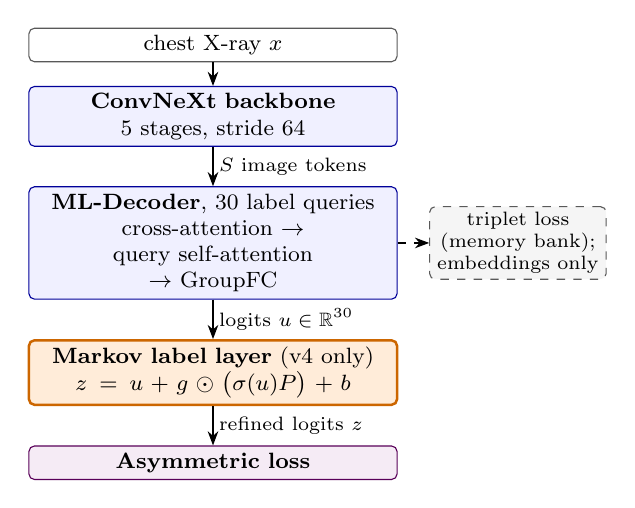
\begin{tikzpicture}[font=\footnotesize, node distance=3mm,
  box/.style={draw=blue!60!black, fill=blue!6, rounded corners=2pt, align=center, text width=4.5cm, inner sep=2.5pt},
  newbox/.style={box, draw=orange!80!black, fill=orange!15, line width=0.9pt},
  lossbox/.style={box, draw=violet!70!black, fill=violet!8},
  databox/.style={box, draw=gray!70!black, fill=white},
  aux/.style={draw=gray!70!black, dashed, fill=gray!8, rounded corners=2pt, align=center, text width=2.1cm, inner sep=2pt, font=\scriptsize},
  arr/.style={-{Stealth[length=1.8mm]}},
  lab/.style={font=\scriptsize, right, inner sep=2pt}]
\node[databox] (x) {chest X-ray $x$};
\node[box, below=of x] (bb) {\textbf{ConvNeXt backbone}\\5 stages, stride 64};
\node[box, below=5mm of bb] (dec) {\textbf{ML-Decoder}, 30 label queries\\cross-attention $\rightarrow$ query self-attention\\$\rightarrow$ GroupFC};
\node[newbox, below=5mm of dec] (mk) {\textbf{Markov label layer} (v4 only)\\$z = u + g \odot \bigl(\sigma(u)P\bigr) + b$};
\node[lossbox, below=5mm of mk] (asl) {\textbf{Asymmetric loss}};
\node[aux, right=4mm of dec] (tri) {triplet loss (memory bank); embeddings only};
\draw[arr] (x) -- (bb);
\draw[arr] (bb) -- node[lab]{$S$ image tokens} (dec);
\draw[arr] (dec) -- node[lab]{logits $u \in \mathbb{R}^{30}$} (mk);
\draw[arr] (mk) -- node[lab]{refined logits $z$} (asl);
\draw[arr, dashed] (dec) -- (tri);
\end{tikzpicture}
\caption{Where the Markov step sits. The baseline (v3) is the model without the orange layer. The post-hoc variants of Sections~\ref{sec:smoothing} and~\ref{sec:gating} act on the probabilities $\sigma(u)$ of a trained v3 model at inference; the trainable layer of Section~\ref{sec:layer} is inserted before the loss and fine-tuned end to end. The post-prediction patient HMM of Section~\ref{sec:hmm} also acts on $\sigma(u)$ of a frozen model, combined with the patient's history and metadata (Fig.~\ref{fig:hmm}).}
\label{fig:pipeline}
\end{figure}

\subsection{Label Transition Matrix}
Let $C_{ij}$ be the number of training images labelled with both $i$ and $j$. The co-occurrence Markov chain has transition matrix
\begin{equation}
P_{ij} = \frac{C_{ij}}{\sum_{k \neq i} C_{ik}}, \quad i \neq j, \qquad P_{ii} = 0,
\label{eq:transition}
\end{equation}
so each row is a probability distribution over the labels that accompany label $i$. $P$ is built from the training fold only. Row normalisation has one unavoidable side effect: the Normal row must also sum to one, so $P$ cannot express that Normal excludes every finding.

\subsection{Post-Hoc Random-Walk Smoothing}
\label{sec:smoothing}
Given an image's predicted probabilities $p \in [0,1]^{30}$, let $s = \sum_c p_c$ and $\hat{p} = p / s$. One random-walk step redistributes the normalised mass along $P$, and we blend it with the original prediction,
\begin{equation}
q = (1 - \alpha)\, p + \alpha\, s\, (\hat{p} P),
\label{eq:smoothing}
\end{equation}
where $\alpha$ sets the strength of the prior. Multiplying by $s$ keeps the total mass of $q$ equal to that of $p$.

\subsection{Normal-Gating}
\label{sec:gating}
The Task~1 winner~\cite{b15} suppresses every abnormal class $c \neq 0$ by the predicted probability $p_0$ of the Normal class,
\begin{equation}
p_c \leftarrow p_c\,(1 - p_0)^{\alpha_{ng}}, \qquad \alpha_{ng} = 0.5.
\label{eq:gating}
\end{equation}
This is a hard-exclusivity prior. In our validation labels, Normal co-occurs with an abnormal finding in only 26 of 17,270 images. We also test a reverse gate that suppresses Normal instead, $p_0 \leftarrow p_0\,(1 - \max_{c \neq 0} p_c)^{0.5}$.

\subsection{Trainable Markov Label Layer}
\label{sec:layer}
A fixed prior cannot adapt to what the network has already learned. We therefore also insert a trainable layer after the logits (Fig.~\ref{fig:layer}):
\begin{align}
P &= \operatorname{softmax}_{\mathrm{row}}\bigl(A \odot (1 - I) - \infty \cdot I\bigr), \label{eq:layerP}\\
z^{(k)} &= u + g \odot \bigl(\sigma(z^{(k-1)})\, P\bigr) + b, \qquad k = 1, \dots, K, \label{eq:layer}
\end{align}
with $z^{(0)} = u$ and output $z = z^{(K)}$. The $30 \times 30$ matrix $A$ is initialised from the log co-occurrence of the training labels, so $P$ starts close to Eq.~\eqref{eq:transition} and stays row-stochastic throughout training. The per-class gate $g$ and bias $b$ start at zero, so the model starts exactly as the baseline and the layer contributes only what training finds useful. The gate is signed: a negative $g_j$ lets co-occurring evidence \emph{lower} the score of label $j$, which is the only way the layer can express exclusivity. The layer has $30 \times 30 + 30 + 30 = 960$ parameters. We train three variants: $K{=}1$ with learnable $A$ (mk1), $K{=}2$ with learnable $A$ (mk2), and $K{=}1$ with $A$ frozen at its co-occurrence initialisation (mk1fix).

\begin{figure}[htbp]
\centering
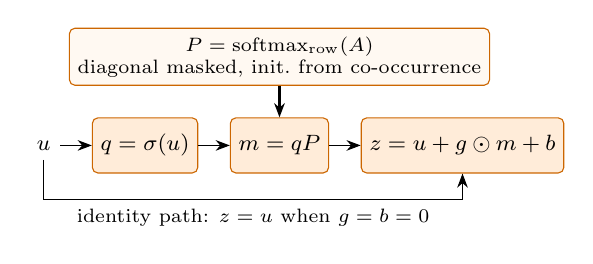
\begin{tikzpicture}[font=\footnotesize, node distance=4mm,
  op/.style={draw=orange!80!black, fill=orange!15, rounded corners=2pt, align=center, inner sep=3pt, minimum height=7mm},
  par/.style={draw=orange!80!black, fill=orange!5, rounded corners=2pt, align=center, inner sep=3pt, font=\scriptsize},
  arr/.style={-{Stealth[length=1.8mm]}}]
\node (u) {$u$};
\node[op, right=of u] (q) {$q = \sigma(u)$};
\node[op, right=of q] (m) {$m = qP$};
\node[op, right=of m] (z) {$z = u + g \odot m + b$};
\node[par, above=4mm of m] (P) {$P = \operatorname{softmax}_{\mathrm{row}}(A)$\\diagonal masked, init.\ from co-occurrence};
\draw[arr] (u) -- (q);
\draw[arr] (q) -- (m);
\draw[arr] (m) -- (z);
\draw[arr, line width=0.9pt] (P) -- (m);
\draw[arr] (u.south) -- ++(0,-5mm) -| node[pos=0.25, below, font=\scriptsize]{identity path: $z = u$ when $g = b = 0$} (z.south);
\end{tikzpicture}
\caption{The trainable Markov label layer for $K{=}1$. $P$ is one global matrix shared by all images; only its input $q$ is image-specific. For $K{=}2$ the step is repeated with $\sigma(z^{(1)})$ in place of $q$.}
\label{fig:layer}
\end{figure}

\subsection{Post-Prediction Patient HMM}
\label{sec:hmm}
For route (B) we keep the classifier frozen and place the Markov model after it, so that the network only extracts image evidence and the patient information enters through the prior.

\textbf{Graphical model.} A patient's studies are grouped into states, one per patient and date (Fig.~\ref{fig:hmm}). The state $y_t \in \{0,1\}^{30}$ is the element-wise OR of the label vectors of that date's studies, and $m_t$ is the date's metadata. The model is a hidden Markov model whose emission is the classifier:
\begin{equation}
p(y_{1:T}, x_{1:T}) = p(y_1 \mid m_1) \prod_{t>1} p(y_t \mid y_{t-1}, m_t) \prod_{t} p(x_t \mid y_t).
\label{eq:hmm}
\end{equation}
The emission can come from any classifier that outputs probabilities; we use the ConvNeXt/ML-Decoder models of Section~\ref{sec:setup}, which have no Mixture-of-Experts head.

\begin{figure}[htbp]
\centering
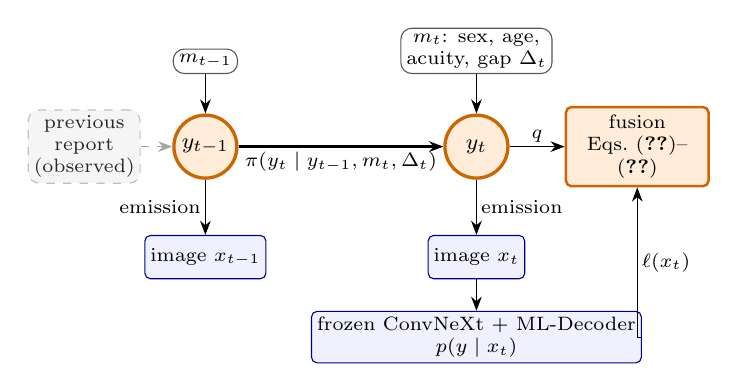
\begin{tikzpicture}[font=\footnotesize,
  st/.style={circle, draw=orange!80!black, fill=orange!15, line width=1.2pt, minimum size=8mm, inner sep=0pt},
  img/.style={draw=blue!60!black, fill=blue!6, rounded corners=2pt, align=center, inner sep=2pt, minimum height=5.5mm, font=\scriptsize},
  meta/.style={draw=gray!70!black, fill=white, rounded corners=4pt, align=center, inner sep=2pt, font=\scriptsize},
  aux/.style={draw=gray!50, dashed, fill=gray!8, rounded corners=4pt, align=center, inner sep=2pt, font=\scriptsize, text=gray!30!black},
  fuse/.style={draw=orange!80!black, fill=orange!15, rounded corners=2pt, align=center, inner sep=3pt, line width=0.9pt, font=\scriptsize},
  arr/.style={-{Stealth[length=1.8mm]}},
  lab/.style={font=\scriptsize, inner sep=1.5pt}]
\node[st] (y0) {$y_{t-1}$};
\node[st, right=26mm of y0] (y1) {$y_t$};
\node[meta, above=5mm of y0] (m0) {$m_{t-1}$};
\node[meta, above=5mm of y1] (m1) {$m_t$: sex, age,\\acuity, gap $\Delta_t$};
\node[aux, left=4mm of y0] (rep) {previous\\report\\(observed)};
\node[img, below=7mm of y0] (x0) {image $x_{t-1}$};
\node[img, below=7mm of y1] (x1) {image $x_t$};
\node[img, below=4mm of x1] (clf) {frozen ConvNeXt + ML-Decoder\\$p(y \mid x_t)$};
\node[fuse, right=7mm of y1, text width=1.6cm] (fz) {fusion\\Eqs.~\eqref{eq:fuse}--\eqref{eq:qw}};
\draw[arr, line width=1.2pt] (y0) -- node[lab, below]{$\pi(y_t \mid y_{t-1}, m_t, \Delta_t)$} (y1);
\draw[arr] (m0) -- (y0);
\draw[arr] (m1) -- (y1);
\draw[arr] (y0) -- node[lab, left]{emission} (x0);
\draw[arr] (y1) -- node[lab, right]{emission} (x1);
\draw[arr, dashed, draw=gray!70] (rep) -- (y0);
\draw[arr] (x1) -- (clf);
\draw[arr] (clf.east) -| node[lab, pos=0.75, right]{$\ell(x_t)$} (fz.south);
\draw[arr] (y1) -- node[lab, above]{$q$} (fz);
\end{tikzpicture}
\caption{The post-prediction patient HMM as a graphical model, with one state per patient and date. Orange circles are the hidden finding states $y_t \in \{0,1\}^{30}$, blue boxes the images and the frozen classifier, white boxes metadata. The transition prior $\pi$ (Eq.~\eqref{eq:trans}) depends on the previous state, the metadata of the current date and the gap $\Delta_t$; a state without an earlier state uses $\pi^{0}(m)$ (Eq.~\eqref{eq:init}). The classifier supplies only the emission (Eq.~\eqref{eq:emission}), and prior and emission are combined after the network. In the observed mode $y_{t-1}$ is read from the previous report (dashed); in the filtered mode it is inferred from $x_{1:t-1}$ by Eqs.~\eqref{eq:predict}--\eqref{eq:update}.}
\label{fig:hmm}
\end{figure}

\textbf{Emission.} The classifier gives posteriors $p_c(x) = P(y_c{=}1 \mid x)$. After a calibration fitted on held-out patients, with a temperature $\tau$ shared by all classes and a per-class intercept $\delta_c$, the posterior is converted into a likelihood ratio by dividing out the training prevalence $\bar\pi_c$:
\begin{equation}
\ell_c(x) = \tau \operatorname{logit} p_c(x) + \delta_c - \operatorname{logit} \bar\pi_c .
\label{eq:emission}
\end{equation}

\textbf{Prior.} The prior factorises over classes, each a logistic model. A state without an earlier state uses $\pi^{0}$; later states use the transition $\pi$:
\begin{align}
\operatorname{logit} \pi^{0}_c(m) &= \alpha^{0}_c + \gamma^{0\top}_c \phi(m), \label{eq:init}\\
\operatorname{logit} \pi_c(y', m, \Delta) &= \alpha_c + \beta_c y'_c + \kappa_c y'_c g + \lambda_c g \nonumber\\
&\quad + \textstyle\sum_{k \neq c} B_{ck}\, y'_k + \gamma_c^{\top} \phi(m), \label{eq:trans}
\end{align}
where $y'$ is the previous state, $g = \log(1 + \Delta)$ for a gap of $\Delta$ days, and $B_{ck}$ is a cross-class temporal edge from class $k$ at the previous state to class $c$ at the current one. The metadata enter as
\begin{equation}
\phi(m) = \bigl[\mathbf{1}_{\mathrm{M}},\ \mathbf{1}_{\mathrm{U}},\ \operatorname{rcs}(\text{age}),\ \mathbf{1}_{\mathrm{AP}},\ \mathbf{1}_{\mathrm{APh}}\bigr],
\label{eq:phi}
\end{equation}
where $\mathbf{1}_{\mathrm{M}}$ and $\mathbf{1}_{\mathrm{U}}$ indicate male and unknown sex, $\operatorname{rcs}$ is a restricted cubic spline of age with knots at the 5th, 35th, 65th and 95th percentiles (three terms), and $\mathbf{1}_{\mathrm{AP}}$ and $\mathbf{1}_{\mathrm{APh}}$ indicate the acuity of the date, an AP or AP horizontal projection against PA or lateral; each column is standardised on the training states. All 30 logistic models are fitted at once, as one batched model in double precision, by L-BFGS on consecutive states of the training fold; $\pi^{0}$ is fitted on the patients' first states. The L2 penalties are chosen by patient-grouped five-fold cross-validated log-loss on the training pairs, and the intercepts $\alpha_c$, $\alpha^0_c$ and the own-state terms $\beta_c$ are not penalised.

\textbf{Fusion.} For a target image $x$ on date $t$,
\begin{align}
z_c &= \tau \operatorname{logit} p_c(x) + \delta_c + w \bigl[\operatorname{logit} q_c - \operatorname{logit} \bar\pi_c\bigr], \label{eq:fuse}\\
(q_c, w) &= \begin{cases}
\bigl(\pi_c(y_{t-1}, m_t, \Delta_t),\ w_h\bigr) & \text{earlier state},\\
\bigl(\pi^{0}_c(m_t),\ w_0\bigr) & \text{otherwise}.
\end{cases} \label{eq:qw}
\end{align}
With $w = 1$ this is Bayes' rule: the prior log-odds plus the emission likelihood ratio of Eq.~\eqref{eq:emission}. We instead fit $w_h$ and $w_0$ on held-out patients, for two reasons: the ASL-trained probabilities are not calibrated posteriors, and the image and the prior can carry the same evidence (a device is both visible in the current image and recorded in the previous report). With $w_h = w_0 = 0$ the model returns the classifier's ranking unchanged.

\textbf{History.} The previous state $y_{t-1}$ can be obtained in two ways (Table~\ref{tab:modes}). In the \emph{observed} mode, it is the label set of the previous report, which a reading radiologist has at hand, and the prior is exactly Eq.~\eqref{eq:trans}. In the \emph{filtered} mode, the previous state is inferred from the patient's earlier images alone by a forward pass with a factorised belief $\mu_t$:
\begin{align}
q_c &= \mu_{t-1,c}\, \sigma\bigl(\eta_c(1, \mu_{t-1})\bigr) \nonumber\\
&\quad + (1 - \mu_{t-1,c})\, \sigma\bigl(\eta_c(0, \mu_{t-1})\bigr), \label{eq:predict}\\
\mu_{t,c} &= \sigma\bigl(\operatorname{logit} q_c + w_e\, \bar\ell_{t,c}\bigr), \label{eq:update}
\end{align}
where $\eta_c(s, \mu)$ is the logit of Eq.~\eqref{eq:trans} with $y'_c = s$ and the other classes at their beliefs, and $\bar\ell_t$ is the mean of Eq.~\eqref{eq:emission} over the images of date $t$. The prediction step is exact when $B = 0$; with cross-class edges it is a mean-field (Boyen--Koller~\cite{b24}) projection. With one-hot beliefs the filtered mode reproduces the observed mode exactly, which our code asserts. At the target date only the target image itself enters; same-date views of other images are not fused, because that would add an unrelated multi-view gain.

\begin{table}[htbp]
\caption{The two history modes of the patient HMM.}
\begin{center}
\footnotesize
\setlength{\tabcolsep}{3pt}
\begin{tabular}{|l|>{\raggedright\arraybackslash}p{2.9cm}|>{\raggedright\arraybackslash}p{3.3cm}|}
\hline
\textbf{Mode} & \textbf{Source of $y_{t-1}$} & \textbf{Prior $q_c$} \\
\hline
observed & labels (0/1) of the previous state's report & $q_c = \pi_c(y_{t-1}, m_t, \Delta_t)$, exact (Eq.~\eqref{eq:trans}) \\
\hline
filtered & belief $\mu_{t-1}$ from a forward pass over all earlier states' images & Eq.~\eqref{eq:predict}, then the update Eq.~\eqref{eq:update}; exact when $B = 0$, mean field otherwise \\
\hline
\end{tabular}
\label{tab:modes}
\end{center}
\end{table}

\textbf{Arms.} The arms add terms in a fixed, pre-specified order (Table~\ref{tab:arms}); H4 is the primary arm. H0 reproduces the late fusion of our earlier study exactly, which our code asserts. Three ablations extend H4.

\begin{table}[htbp]
\caption{Arms of the patient HMM. Each arm adds to the one above it; H4 is the pre-specified primary arm, and H5, H4-acq and H4-F are ablations of it.}
\begin{center}
\footnotesize
\setlength{\tabcolsep}{3pt}
\begin{tabular}{|l|>{\raggedright\arraybackslash}p{6.6cm}|}
\hline
\textbf{Arm} & \textbf{Adds} \\
\hline
E & the emission only ($w_h = w_0 = 0$) \\
H0 & pooled per-class two-state chain, $a_c = P(1 \mid 1)$ and $b_c = P(1 \mid 0)$ with Laplace smoothing; $w_h = 1$, no calibration. Reproduces the late fusion of our earlier study exactly \\
H1 & $+$ calibration ($\tau$, $\delta$) and a cross-fitted $w_h$ \\
H2 & $+$ gap terms $\kappa$, $\lambda$ \\
H3 & $+$ metadata $\phi(m)$ in $\pi$ and $\pi^{0}$; $w_0$ then also changes images without an earlier state \\
\textbf{H4} & $+$ cross-class temporal edges $B_{ck}$ (class $k$ at $t-1$ to class $c$ at $t$) \\
\hline
H5 & $+$ within-state label couplings $J$: a pairwise Markov random field fitted by pseudo-likelihood, applied by damped mean field with a fitted weight $w_J$ \\
H4-acq & $+$ per-state DICOM acquisition fields in $\phi$ (care-setting proxies) \\
H4-F & H4 in the filtered mode \\
\hline
\end{tabular}
\label{tab:arms}
\end{center}
\end{table}

\textbf{In-network comparator (B-early).} The alternative is to give the network the same prior. B-early maps the pooled-chain prior vector $\bigl[\operatorname{logit} \pi_c(y_{t-1}) - \operatorname{logit} \bar\pi_c\bigr]_{c} \oplus \mathbf{1}[\text{earlier state}]$, through two zero-initialised linear maps, to an offset on the 30 ML-Decoder label queries. It is fine-tuned with the baseline recipe (prior dropout 0.3) at seeds 42 and 1024, and starts exactly as the baseline. B-early0 is the same network evaluated with every prior set to zero, the only condition available on the test set.

\section{Experimental Setup}
\label{sec:setup}
\textbf{Data.} We use the CXR-LT 2026 Task~1 training data: PadChest~\cite{b9} images with 30 report-derived target labels, split into an internal training fold (103,303 images after filtering) and a validation fold (17,270 scored images). Patient identifiers, study identifiers and projections come from the original PadChest metadata.

\textbf{Post-hoc experiments.} Sections~\ref{sec:smoothing} and~\ref{sec:gating} are evaluated on cached validation probabilities with horizontal-flip test-time augmentation (TTA). The base model is our best greedy three-model ensemble: two SWA checkpoints (768~px, seed 42; 1024~px, seed 86) and one best-epoch checkpoint (640~px, seed 86). The metric is macro mAP over the 30 classes. No model is retrained.

\textbf{Trainable-layer experiments.} Each variant fine-tunes from the same Stage-1 checkpoint with our final Stage-2 recipe: 768~px input, seed 42, drop-path 0.1, four epochs of an eight-epoch cosine schedule, effective batch size 48, triplet weight $\lambda = 0.1$ and a memory bank of 2,048 embeddings. The baseline is the identical run without the layer. $A$, $g$ and $b$ are trained with a learning rate ten times the base rate ($10^{-3}$ versus $10^{-4}$) and no weight decay, because $g$ and $b$ start from zero. We report the best epoch of the EMA weights and the stochastic weight average (SWA) of the EMA weights over the last three epochs.

\textbf{Metadata analysis.} We relate PadChest patient, study and acquisition metadata to the 30 labels on the training fold only (50,604 patients, 75,819 studies). Labels come from the challenge label lists, never from the PadChest report or label columns, and only a whitelist of metadata columns is read, for training and validation images only. Patient and study fields (sex, age at study, pediatric flag, number of earlier states, days since the previous study, study year, study acuity) are counted per study; view and acquisition fields (projection, scanner manufacturer, spatial resolution, exposure, image size and others) are counted per image. For each field and class we compute Cram\'er's V, mutual information, a chi-square test with Benjamini--Hochberg correction, and the log odds ratio of the most extreme level with a patient-clustered bootstrap interval (200 resamples). The tests ignore the clustering of studies within patients, so we rank by effect size. A per-class logistic regression on metadata alone is scored by patient-grouped five-fold cross-validation, with each feature group (patient: sex and age; temporal; view; acquisition) alone and removed in turn. To test whether metadata add to the image model, we fit on the validation fold, for each class, a logistic model of the label on the image logit plus the metadata, fitted on one half of the patients and scored on the other (both directions). We compute mAP within each half, average the two, and compare with the unmodified image probabilities by a paired patient-clustered bootstrap (300 resamples). The image models are the 768~px seed-42 SWA model and the greedy three-model ensemble, both with flip TTA.

\textbf{Longitudinal simulation.} Route (B) is evaluated on the internal folds only, as a simulation of reading with prior studies; no development or test image is ever linked to the PadChest metadata, and only a whitelist of metadata columns is read (dates, projection, sex and birth year, plus acquisition fields for H4-acq), never the report or label columns. The prior is fitted on training-fold states only (74,782 states, 24,180 consecutive pairs). Validation images take their history from both folds, as in a hospital archive: 5,759 of the 17,270 have an earlier state, and the primary subset is the 4,061 of these that are frontal. Calibration and fusion weights are cross-fitted: the validation patients are split into two halves, all parameters are fitted on one half (the weights by macro mAP on the grid $\{0, 0.25, \dots, 1.5\}$) and applied to the other, for three random splits. Because the halves receive different calibrations, AP is computed within each half and averaged; pooling them would mix two scales inside each class ranking. The emissions are the 768~px SWA models at seeds 42 and 1024 and the greedy ensemble, all with flip TTA, and B-early is compared with the emission of the same seed. In the filtered mode, training-fold images have in-sample emissions from the seed-42 model (mAP 0.713 on the training fold), so a filtered history built from training images is optimistic. Differences use a paired patient-clustered bootstrap of 300 resamples on the first split.

\textbf{Validation subsets.} To compare with the test set, we split the validation fold by projection (frontal: PA, AP and AP horizontal; lateral) and by whether the image's patient also appears in the training fold. Scores on a subset are macro mAP over the classes with at least one positive in that subset (28 classes for the frontal, unseen-patient subset). The cached probabilities carry no sample keys, so we rebuilt their row order from the evaluation data-loader schedule; the rebuilt order reproduces all 17,270 stored label rows exactly, and only one arrangement of the four images missing from the shards fits. Differences between two models are tested with a patient-clustered bootstrap of 300 resamples.

\section{Results}

\subsection{Random-Walk Smoothing}
Table~\ref{tab:smoothing} shows that smoothing lowers mAP at every strength, and the loss grows with $\alpha$. At $\alpha = 0.05$ the loss falls mainly on the head classes: the mean change in per-class AP is $-0.0021$ over the ten most frequent classes and $-0.0001$ over the ten rarest.

\begin{table}[htbp]
\caption{Post-hoc random-walk smoothing (Eq.~\eqref{eq:smoothing}) on the greedy-3 ensemble, flip TTA, $n_{val} = 17{,}270$.}
\begin{center}
\begin{tabular}{|c|c|c|}
\hline
$\boldsymbol{\alpha}$ & \textbf{mAP} & \textbf{$\Delta$ vs base} \\
\hline
0 (base) & \textbf{0.4722} & --- \\
\hline
0.02 & 0.4716 & $-0.0006$ \\
\hline
0.05 & 0.4710 & $-0.0012$ \\
\hline
0.10 & 0.4698 & $-0.0024$ \\
\hline
0.20 & 0.4669 & $-0.0053$ \\
\hline
\end{tabular}
\label{tab:smoothing}
\end{center}
\end{table}

AP is a per-class ranking metric. Smoothing moves probability from an image's confident findings to findings that accompany them \emph{on average}, which blurs the per-image evidence the ranking depends on. The ML-Decoder already learns label interactions through its queries, so a fixed co-occurrence prior adds no new information.

\subsection{Normal-Gating}
Normal-gating lowers mAP at every strength (Table~\ref{tab:gating}), and 28 of 30 classes get worse. The single 1024~px model behaves the same way ($-0.024$ at $\alpha_{ng} = 0.5$). The reverse gate leaves mAP unchanged. The winner trained with a Distribution-Balanced loss~\cite{b23} and class-aware sampling, both of which push abnormal scores up, and used the gate to \emph{``suppress spurious abnormal predictions''}~\cite{b15}. Our Asymmetric-Loss model has no such bias, so the gate only spreads the errors in $p_0$ into every other class's ranking. This comparison uses report-derived labels; the leaderboard uses radiologist labels.

\begin{table}[htbp]
\caption{Normal-gating (Eq.~\eqref{eq:gating}) on the greedy-3 ensemble, flip TTA.}
\begin{center}
\begin{tabular}{|l|c|c|}
\hline
\textbf{Variant} & \textbf{mAP} & \textbf{$\Delta$} \\
\hline
base & \textbf{0.4722} & --- \\
\hline
gate, $\alpha_{ng} = 0.25$ & 0.4619 & $-0.0103$ \\
\hline
gate, $\alpha_{ng} = 0.5$ (winner's setting) & 0.4483 & $-0.0239$ \\
\hline
gate, $\alpha_{ng} = 1.0$ & 0.4264 & $-0.0459$ \\
\hline
reverse gate on Normal & 0.4722 & $\pm 0.0000$ \\
\hline
\end{tabular}
\label{tab:gating}
\end{center}
\end{table}

\subsection{Trainable Markov Label Layer}
\label{sec:layerres}
None of the three variants improves on the matched baseline (Table~\ref{tab:layer}). Best-epoch mAP changes by $-0.0044$ (mk1), $-0.0000$ (mk2) and $-0.0016$ (mk1fix), and SWA mAP by $-0.0049$, $-0.0033$ and $-0.0031$. mAUC and mECE stay within 0.001 of the baseline, and mF1 moves in both directions. The SWA shortfall is consistent in sign but small against seed noise. Over six seeds of our 512~px recipe, best-epoch mAP spans 0.0065 (standard deviation about 0.0031), and two seeds of the 768~px baseline recipe differ by 0.0021 (best epoch) and 0.0018 (SWA). With one seed per variant, we cannot tell no effect from a slight harm, or rank the variants against each other.

\begin{table*}[htbp]
\caption{Trainable Markov label layer versus the matched baseline (768~px, seed 42, no TTA). Best: EMA weights at the best epoch. SWA: average of the EMA weights of epochs 2--4; mAUC, mF1 and mECE are for the SWA weights. $|g|$: mean / max absolute gate after the final epoch.}
\begin{center}
\begin{tabular}{|l|c|c|c|c|c|c|c|c|}
\hline
\textbf{Model} & $\boldsymbol{K}$ & $\boldsymbol{A}$ & \textbf{Best mAP} & \textbf{SWA mAP} & \textbf{mAUC} & \textbf{mF1} & \textbf{mECE} & $\boldsymbol{|g|}$ \\
\hline
Baseline (v3) & --- & --- & \textbf{0.4585} & \textbf{0.4600} & 0.9092 & 0.4685 & 0.1354 & --- \\
\hline
mk1 & 1 & learned & 0.4541 & 0.4551 & 0.9096 & 0.4661 & 0.1360 & 0.013 / 0.061 \\
\hline
mk2 & 2 & learned & \textbf{0.4585} & 0.4566 & 0.9097 & 0.4719 & 0.1354 & 0.011 / 0.047 \\
\hline
mk1fix & 1 & frozen & 0.4569 & 0.4569 & 0.9088 & 0.4642 & 0.1353 & 0.013 / 0.061 \\
\hline
\end{tabular}
\label{tab:layer}
\end{center}
\end{table*}

The gates show why. Starting from zero, the mean $|g|$ grew slowly and steadily to 0.011--0.013 by the fourth epoch, with a maximum of 0.047--0.061. The gate statistics are nearly identical whether $A$ is learned or frozen, and the learned $A$ moved little from its initialisation. Even with ten times the base learning rate, training kept the layer close to the identity. We have not tested whether a larger learning-rate multiplier or a longer schedule would change this. These checkpoints were not evaluated with TTA, per class, or on the validation subsets of Section~\ref{sec:audit}.

\subsection{Longitudinal Markov Model}
\label{sec:hmmres}
Locally, the longitudinal structure exists. In the PadChest metadata, 13,198 of 50,604 training patients have at least two studies, covering 50.1\% of training images; in the validation fold, 1,548 of 14,501 patients do, covering 21.6\% of images. At test time, however, there is nothing to condition on. The challenge organisers state that \emph{``because PadChest-GR is derived from PadChest, we performed both patient-level and study-level de-duplication to prevent leakage''} and that \emph{``patient identifiers and hidden evaluation labels were not released to participants''}~\cite{b14}. Test patients therefore have no history in the training data. Test images remain linkable in principle to the public PadChest metadata, but participants must follow \emph{``the applicable data-use restrictions, including research-only use, no redistribution, and no attempts to re-identify individual patients''}~\cite{b14}, so building a history this way would breach the terms. We did not attempt it. A longitudinal model is only meaningful in a deployment study with genuine prior studies, the setting of the temporal work in Section~II, which targets progression labels rather than Task~1's static findings.

We nevertheless measure what such a model would do, as a simulation on the internal folds (Section~\ref{sec:hmm}); the leaderboard effect is 0 by construction. Table~\ref{tab:hmm} gives the results, and every difference is relative to the unmodified emission E.

\textbf{Main result.} The primary arm H4 raises mAP on validation images that have an earlier state and are frontal (the primary subset, $n = 4{,}061$) by $+0.0375$ (95\% CI $+0.0228$ to $+0.0513$) with the 768~px seed-42 model and by $+0.0424$ ($+0.0279$ to $+0.0592$) with the seed-1024 model; the three-model ensemble gives $+0.0364$ ($+0.0209$ to $+0.0517$). On the primary subset, mAP goes from 0.502 to 0.541 for seed 42 (mean over three splits). On images with an earlier state, the gain is largest for medium and tail classes ($+0.044$ and $+0.046$ against $+0.013$ for head classes at seed 42, with the CXR-LT frequency groups of 3 head, 20 medium and 7 tail classes), as expected if it comes from findings that persist between visits. Calibration also repairs the probabilities: mECE falls from 0.135 to 0.007.

\textbf{H4 versus B-early.} The paired difference between H4 and the network that is fed the same prior (B-early) is $+0.0021$ ($-0.0155$ to $+0.0197$) at seed 42 and $-0.0022$ ($-0.0204$ to $+0.0158$) at seed 1024 on the primary subset, and $-0.0037$ and $-0.0022$ on the full validation fold; every interval includes 0. A model that is retrained with the prior therefore gains nothing over fusing the prior after the classifier, which needs no retraining. Evaluated with its prior set to zero, the only condition possible on the test set, B-early is no better than E ($-0.0027$ and $+0.0004$ on the full fold).

\textbf{The simplest arm is best.} Adding terms to the chain does not help (Table~\ref{tab:hmm}). H1, which only adds the calibration and a fitted weight $w_h$ to the pooled chain, has the highest mAP on every subset with a prior, at all three emissions (primary subset: 0.5511 against 0.5411 for H4 at seed 42). The gap (H2), metadata (H3), cross-class edges (H4), a within-state random field (H5) and acquisition fields (H4-acq) each add nothing, although the held-out transition prior improves with each of them (macro AUROC 0.66, 0.76, 0.80 and 0.81 for the table, gap, metadata and cross-class models; log-loss 0.1513 to 0.1370). The reason is the one given in Section~\ref{sec:metaeda}: metadata are redundant with the image, and the image already shows what the prior would add. Without the calibration (H0, which reproduces the late fusion of our earlier study), the gain is smaller ($+0.0354$ and $+0.0425$ on the primary subset) and the full-fold change is not significant. The H1 comparisons with B-early are exploratory: $+0.0124$ ($-0.0076$ to $+0.0348$) at seed 42 and $+0.0081$ ($-0.0126$ to $+0.0285$) at seed 1024 on the primary subset.

\textbf{Filtered mode.} Most of the gain needs the previous report. When the previous state is inferred from the patient's earlier images instead of read from the report (H4-F, seed 42), the primary-subset gain falls from $+0.0375$ to $+0.0092$ ($-0.0013$ to $+0.0181$), about a quarter. On the 248 images whose history is entirely out-of-sample it is $+0.0043$ ($-0.0098$ to $+0.0187$). The filtered history of training images uses in-sample emissions (training mAP 0.713 against about 0.465 on validation), so this figure is if anything optimistic. A model that copies the previous report would give the same pattern, and so would genuine persistence of findings; we cannot separate the two with report-derived labels. H4-F is clearly below B-early on the primary subset ($-0.0265$, $-0.0467$ to $-0.0063$, exploratory).

\textbf{Ablations.} The random field (H5) selected its weight $w_J = 0$ in every fold, so H5 equals H4 to four decimals. The strongest within-state couplings it learned are among Normal and pleural effusion ($-1.51$), cardiomegaly ($-1.40$) and Support Devices ($-1.31$), and between Support Devices and central venous catheters ($+1.46$): label correlations that the ML-Decoder head already uses. Acquisition fields (H4-acq) leave the primary-subset gain unchanged ($+0.0377$ against $+0.0375$ at seed 42; $+0.0431$ against $+0.0424$ at seed 1024), although they lower the prior's held-out log-loss from 0.1370 to 0.1346 and raise its AUROC from 0.813 to 0.836. The largest learned cross-class edges are negative from Normal or a sternotomy to a new finding in the next study ($-0.86$ for sternotomy to Normal, $-0.85$ for Normal to pleural effusion).

\textbf{Guards and copy check.} On images with no earlier state, H4 is slightly worse than E at seed 42 ($-0.0009$, $-0.0018$ to $-0.0001$) and neutral at seed 1024 ($-0.0005$, $-0.0015$ to $+0.0005$); H1 leaves these images unchanged. A copy check on findings that are new relative to the previous report (28 classes) shows a small drop in AP for H4 (0.3678 to 0.3621 at seed 42, 0.3647 to 0.3615 at seed 1024; no interval computed). Thus the gain is not bought on new findings, but the prior does not help them either, and the H4 guards are met only approximately. On patients unseen in training, H4 changes mAP by $-0.0053$ ($-0.0151$ to $-0.0006$) at seed 42. Why metadata add nothing is shown in Section~\ref{sec:metaeda}.

\begin{table*}[htbp]
\caption{Post-prediction patient HMM on the internal validation fold: change in macro mAP relative to the emission E (the frozen 768~px SWA model with flip TTA; the E row gives absolute mAP). Primary = frontal images with an earlier state ($n = 4{,}061$); full = 17,270 images; no\_prior = 11,511 images without an earlier state. mAP is computed within each of two patient halves (calibration and fusion weights are fitted on one half and applied to the other) and averaged, over three random splits. Each entry is the mean difference with a 95\% CI from a paired patient-clustered bootstrap (300 resamples) on the first split. Entries marked $^\dagger$ (H2, H5) have no bootstrap: they are differences of the three-split mean mAP and are not comparable to the other entries at the 0.001 level. H4-F (image-only history) was run for seed 42 only; B-early and B-early0 are the in-network comparator with and without its prior. This is an internal longitudinal simulation with report-derived history; its leaderboard effect is 0. Results for the three-model ensemble are given in the text.}
\begin{center}
\footnotesize
\setlength{\tabcolsep}{3pt}
\begin{tabular}{|l|c|c|c|c|c|c|}
\hline
 & \multicolumn{3}{c|}{\textbf{Seed 42 (768~px)}} & \multicolumn{3}{c|}{\textbf{Seed 1024 (768~px)}} \\
\textbf{Arm} & full & primary & no\_prior & full & primary & no\_prior \\
\hline
E (absolute mAP) & 0.4652 & 0.5020 & 0.4543 & 0.4635 & 0.4937 & 0.4551 \\
\hline
H0 & \shortstack{+0.0090\\{[$-$0.0033,+0.0242]}} & \shortstack{+0.0354\\{[+0.0150,+0.0583]}} & 0 (identical) & \shortstack{+0.0115\\{[$-$0.0003,+0.0274]}} & \shortstack{+0.0425\\{[+0.0222,+0.0669]}} & 0 (identical) \\
H1 & \shortstack{+0.0222\\{[+0.0135,+0.0353]}} & \shortstack{+0.0477\\{[+0.0298,+0.0664]}} & 0 (identical) & \shortstack{+0.0259\\{[+0.0165,+0.0396]}} & \shortstack{+0.0527\\{[+0.0346,+0.0752]}} & 0 (identical) \\
H2 & +0.0197$^\dagger$ & +0.0460$^\dagger$ & 0$^\dagger$ & +0.0202$^\dagger$ & +0.0521$^\dagger$ & 0$^\dagger$ \\
H3 & \shortstack{+0.0160\\{[+0.0093,+0.0239]}} & \shortstack{+0.0378\\{[+0.0226,+0.0516]}} & \shortstack{$-$0.0009\\{[$-$0.0018,$-$0.0001]}} & \shortstack{+0.0167\\{[+0.0101,+0.0250]}} & \shortstack{+0.0435\\{[+0.0290,+0.0612]}} & \shortstack{$-$0.0005\\{[$-$0.0015,+0.0005]}} \\
H4 & \shortstack{+0.0152\\{[+0.0089,+0.0226]}} & \shortstack{+0.0375\\{[+0.0228,+0.0513]}} & \shortstack{$-$0.0009\\{[$-$0.0018,$-$0.0001]}} & \shortstack{+0.0158\\{[+0.0090,+0.0245]}} & \shortstack{+0.0424\\{[+0.0279,+0.0592]}} & \shortstack{$-$0.0005\\{[$-$0.0015,+0.0005]}} \\
H5 & +0.0160$^\dagger$ & +0.0390$^\dagger$ & $-$0.0003$^\dagger$ & +0.0168$^\dagger$ & +0.0459$^\dagger$ & $-$0.0002$^\dagger$ \\
H4-acq & \shortstack{+0.0174\\{[+0.0111,+0.0247]}} & \shortstack{+0.0377\\{[+0.0230,+0.0515]}} & \shortstack{$-$0.0001\\{[$-$0.0026,+0.0023]}} & \shortstack{+0.0177\\{[+0.0117,+0.0249]}} & \shortstack{+0.0431\\{[+0.0287,+0.0599]}} & \shortstack{+0.0011\\{[$-$0.0025,+0.0045]}} \\
H4-F & \shortstack{+0.0032\\{[$-$0.0016,+0.0083]}} & \shortstack{+0.0092\\{[$-$0.0013,+0.0181]}} & \shortstack{$-$0.0009\\{[$-$0.0018,$-$0.0001]}} & \multicolumn{3}{c|}{not run} \\
B-early & \shortstack{+0.0191\\{[+0.0129,+0.0257]}} & \shortstack{+0.0339\\{[+0.0152,+0.0554]}} & \shortstack{+0.0014\\{[$-$0.0045,+0.0130]}} & \shortstack{+0.0185\\{[+0.0106,+0.0246]}} & \shortstack{+0.0436\\{[+0.0254,+0.0632]}} & \shortstack{+0.0002\\{[$-$0.0058,+0.0062]}} \\
B-early0 & \shortstack{$-$0.0027\\{[$-$0.0092,+0.0047]}} & \shortstack{$-$0.0071\\{[$-$0.0197,+0.0013]}} & \shortstack{+0.0014\\{[$-$0.0045,+0.0130]}} & \shortstack{+0.0004\\{[$-$0.0045,+0.0049]}} & \shortstack{0.0000\\{[$-$0.0074,+0.0091]}} & \shortstack{+0.0002\\{[$-$0.0058,+0.0062]}} \\
\hline
\end{tabular}
\label{tab:hmm}
\end{center}
\end{table*}

\subsection{Patient Metadata and Findings}
\label{sec:metaeda}
\textbf{Associations.} Many fields are associated with the labels (Fig.~\ref{fig:assoc}). The strongest are the acuity of the study (maximum Cram\'er's $V$ 0.528), the projection (0.504), age (0.447) and the time since the previous study (0.447), followed by scanner resolution and exposure fields ($V$ up to 0.406). Sex is weak (maximum $V$ 0.133). The devices are tied to the care setting: Support Devices and central venous catheters occur far more often in portable AP-horizontal studies (log odds ratio $+2.95$ and $+3.52$) and after short gaps. Age drives the other findings (Fig.~\ref{fig:age}): Normal falls from about 70\% of studies below 40 years to about 10\% above 90, while cardiomegaly, aortic elongation, aortic atheromatosis and pleural effusion rise steeply. The single-feature AUROC of age is 0.816 for aortic atheromatosis and 0.776 for aortic elongation. The associations of the tail classes are weak and rest on few positives.

\textbf{Metadata alone.} Metadata predict the labels well above chance. Held-out macro AUROC is 0.760 (chance 0.5) and macro AP is 0.142 (prevalence 0.050); the best classes are central venous catheter (AUROC 0.93) and Support Devices (0.90), and the worst are azygos lobe (0.61) and hypoexpansion (0.64) (Fig.~\ref{fig:auroc}, Table~\ref{tab:metaonly}). Removing the patient fields costs the most (macro AUROC $0.760 \to 0.691$). The acquisition fields rank second, but they identify the scanner and care setting, such as portable AP-supine units, and not patient biology. The AUROCs of the tail classes rest on a handful of positives and are unstable.

\begin{table}[htbp]
\caption{Metadata-only logistic model, patient-grouped five-fold cross-validation on the training fold. Macro average over the 30 classes. Chance: AUROC 0.5, AP 0.050 (mean prevalence).}
\begin{center}
\begin{tabular}{|l|c|c|}
\hline
\textbf{Features} & \textbf{AUROC} & \textbf{AP} \\
\hline
All groups & 0.760 & 0.142 \\
\hline
Patient only & 0.654 & 0.088 \\
\hline
Temporal only & 0.589 & 0.090 \\
\hline
View only & 0.589 & 0.082 \\
\hline
Acquisition only & 0.659 & 0.091 \\
\hline
All $-$ patient & 0.691 & 0.116 \\
\hline
All $-$ temporal & 0.752 & 0.130 \\
\hline
All $-$ view & 0.753 & 0.139 \\
\hline
All $-$ acquisition & 0.729 & 0.133 \\
\hline
\end{tabular}
\label{tab:metaonly}
\end{center}
\end{table}

\textbf{Metadata add nothing to the image.} Stacking metadata on the image logit lowers mAP in every cell (Table~\ref{tab:incr}). On all validation images, the patient fields change mAP by $-0.0026$ (seed 42) and $-0.0049$ (ensemble), and all three groups together by $-0.0095$ and $-0.0123$. On frontal images the changes are similar. The 95\% intervals exclude zero in 15 of 16 cells. This is not a calibration artefact: refitting only a per-class slope and intercept changes mAP by $0.0000$ (seed 42) and $-0.0003$ (ensemble). The image already shows devices, age-related aortic change and the AP-supine geometry, so the metadata add only noise.

\begin{table*}[htbp]
\caption{Change in validation mAP when metadata are stacked on the image logit (cross-fitted on patient halves; 95\% patient-clustered bootstrap interval in brackets). Base: mAP of the image model alone, averaged over the two halves. s42: 768~px seed-42 SWA model; ens: greedy three-model ensemble; both with flip TTA.}
\begin{center}
\footnotesize
\setlength{\tabcolsep}{2.1pt}
\begin{tabular}{|l|l|c|c|c|c|c|}
\hline
\textbf{Model} & \textbf{Images} & \textbf{Base} & \textbf{+ patient} & \textbf{+ view} & \textbf{+ acquisition} & \textbf{+ all three} \\
\hline
s42 & all & 0.4687 & $-0.0026$ [$-0.0047$, $-0.0004$] & $-0.0036$ [$-0.0075$, $-0.0008$] & $-0.0048$ [$-0.0079$, $-0.0018$] & $-0.0095$ [$-0.0138$, $-0.0056$] \\
\hline
s42 & frontal & 0.4940 & $-0.0028$ [$-0.0050$, $-0.0010$] & $-0.0032$ [$-0.0081$, $+0.0022$] & $-0.0063$ [$-0.0120$, $-0.0018$] & $-0.0106$ [$-0.0174$, $-0.0049$] \\
\hline
ens & all & 0.4785 & $-0.0049$ [$-0.0083$, $-0.0023$] & $-0.0047$ [$-0.0089$, $-0.0019$] & $-0.0069$ [$-0.0110$, $-0.0034$] & $-0.0123$ [$-0.0181$, $-0.0076$] \\
\hline
ens & frontal & 0.5062 & $-0.0060$ [$-0.0153$, $-0.0012$] & $-0.0044$ [$-0.0087$, $-0.0010$] & $-0.0091$ [$-0.0181$, $-0.0031$] & $-0.0158$ [$-0.0264$, $-0.0067$] \\
\hline
\end{tabular}
\label{tab:incr}
\end{center}
\end{table*}

\textbf{Transitions depend on acuity.} In consecutive studies of the same patient (24,180 pairs from the training fold), the chance that a finding persists depends on the acuity of the later study (Fig.~\ref{fig:persist}). Devices and catheters persist more after an AP study: Support Devices 0.578 for PA or lateral studies against 0.834 for AP-horizontal, and central venous catheter 0.269 against 0.812. Normal persists less: 0.676 against 0.258. Sex changes mean persistence by less than 0.01 (0.468 for women, 0.459 for men). The AP cells are small and the per-class values are noisy.

\textbf{Consequence.} Metadata are informative about the findings but redundant with the image. In a longitudinal model they should therefore enter, if at all, through the transition between studies, where acuity and the time gap change persistence, and not as a per-image prior. The labels are derived from reports, so some associations reflect reporting habits. Our validation fold is not patient-disjoint (Section~\ref{sec:audit}). No metadata or history exist for the leaderboard test images and joining them to PadChest is not permitted, so none of these results can change the leaderboard score: the effect there is zero by construction.

\begin{figure*}[htbp]
\centering
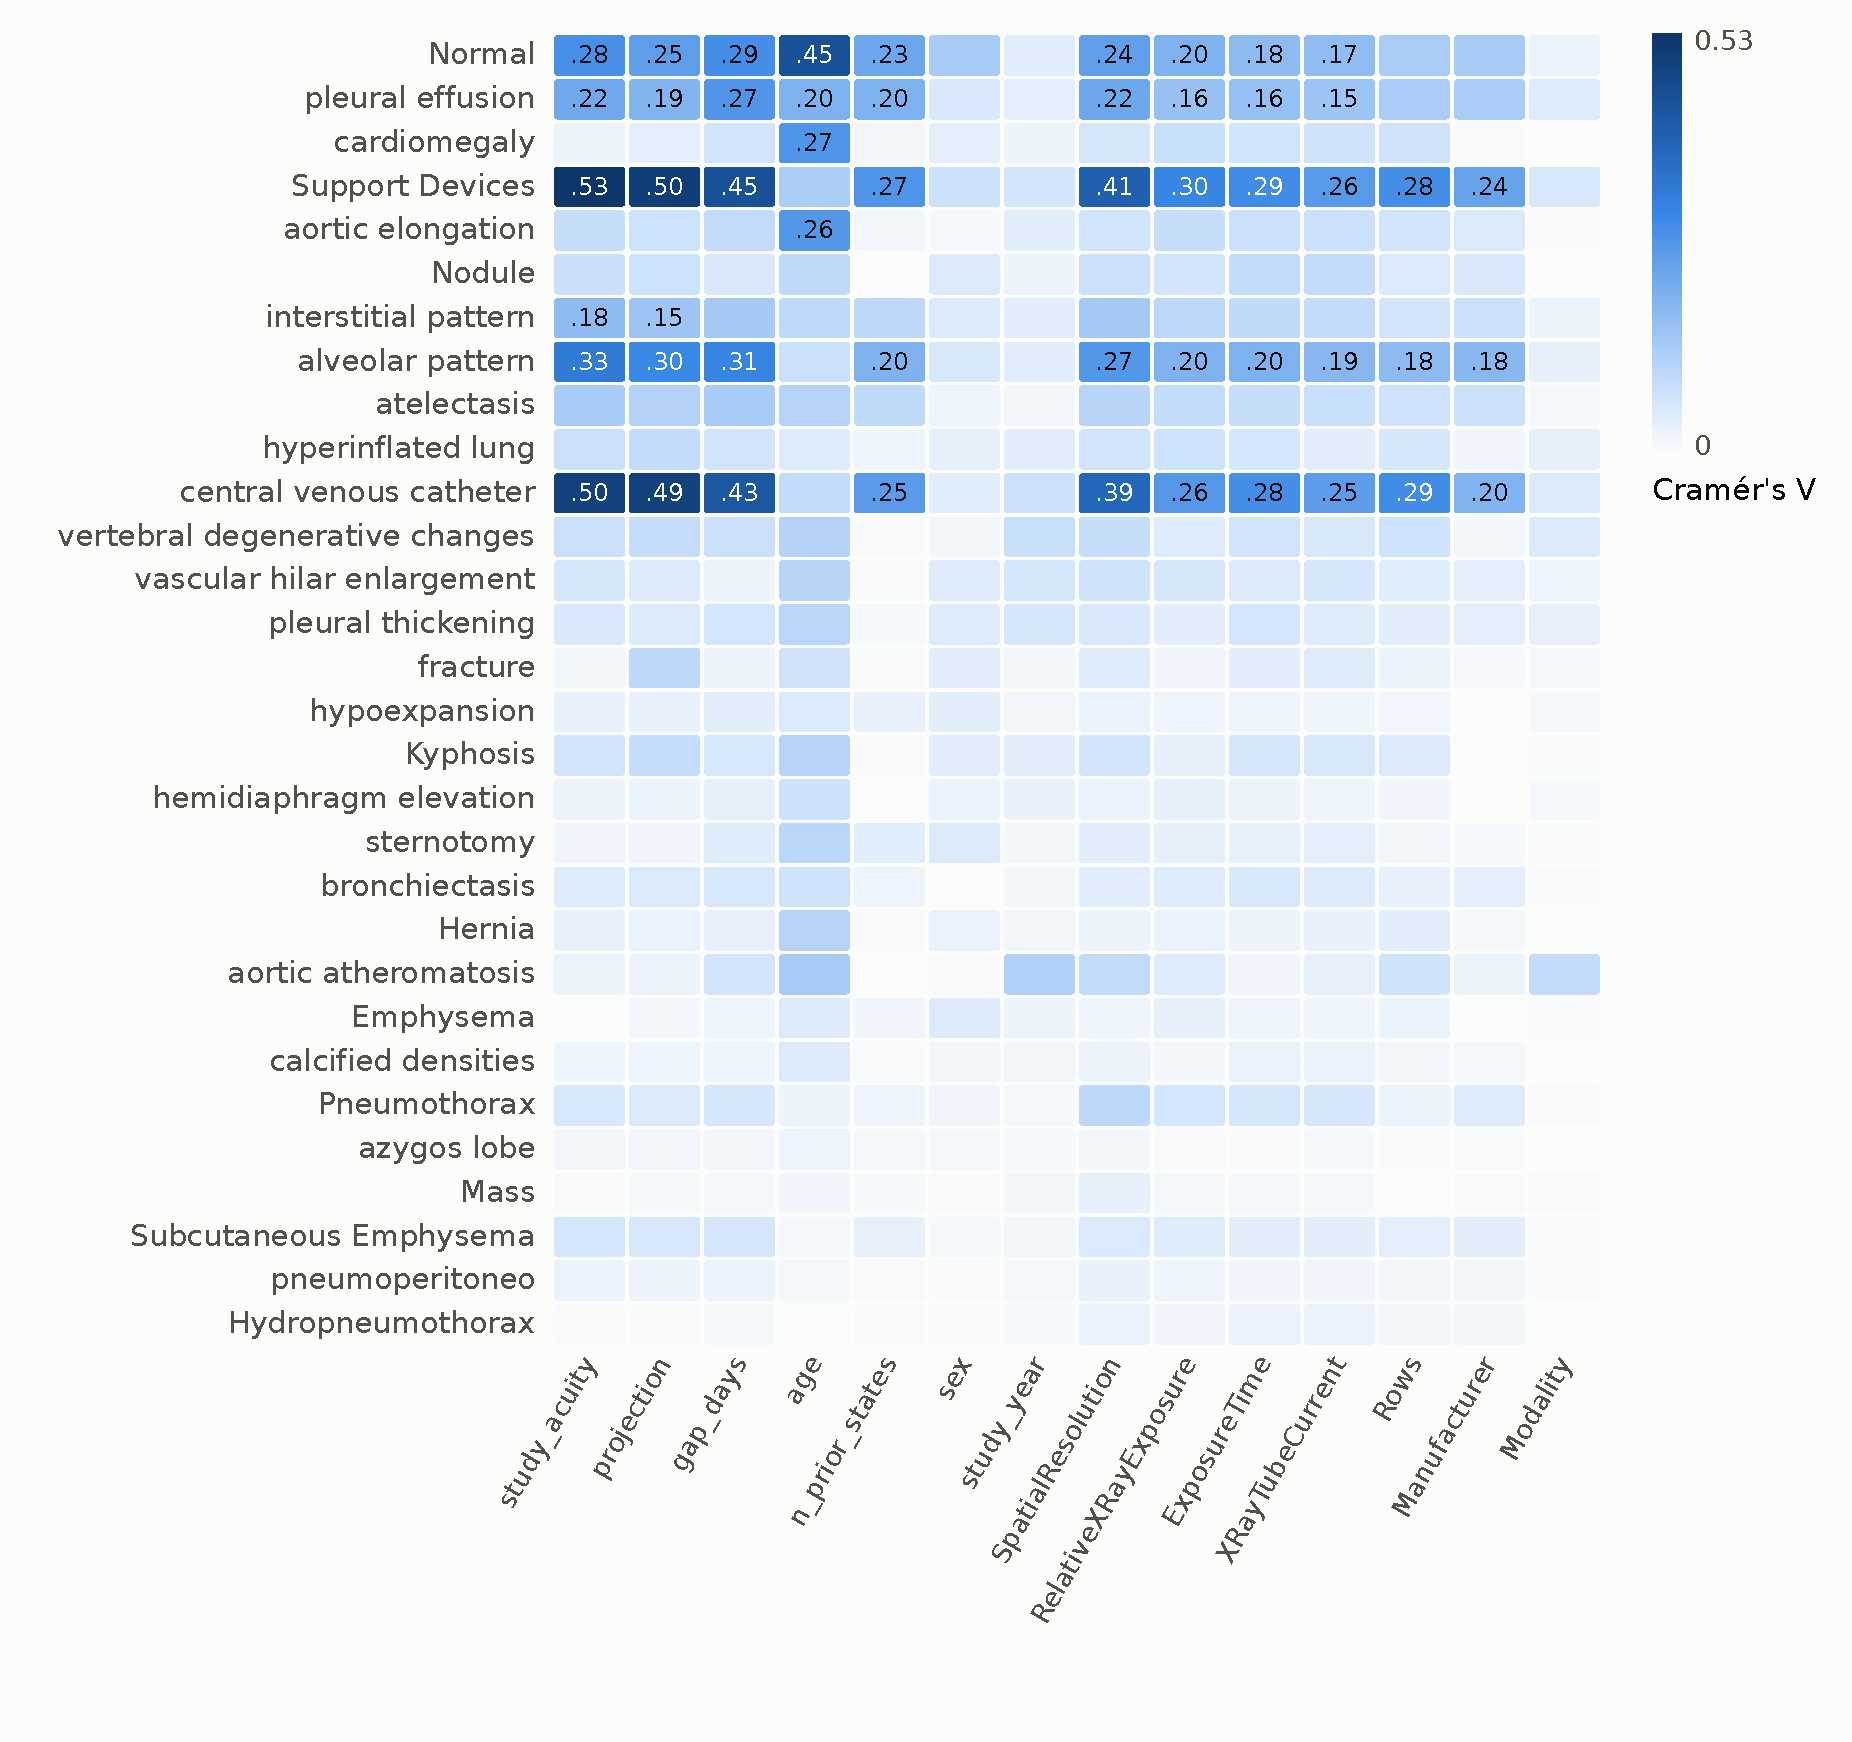
\includegraphics[width=\textwidth]{figures/assoc_heatmap.pdf}
\caption{Association between metadata fields (columns) and the 30 labels (rows, ordered by training prevalence, most frequent at the top) on the training fold. Colour is Cram\'er's $V$ from white (0) to dark blue (0.53); values of 0.15 and above are printed. The study-level fields are acuity, projection, time gap, age, number of earlier studies, sex and year; the remaining columns are acquisition fields (scanner resolution, relative exposure, exposure time, tube current, image rows, manufacturer, modality).}
\label{fig:assoc}
\end{figure*}

\begin{figure*}[htbp]
\centering
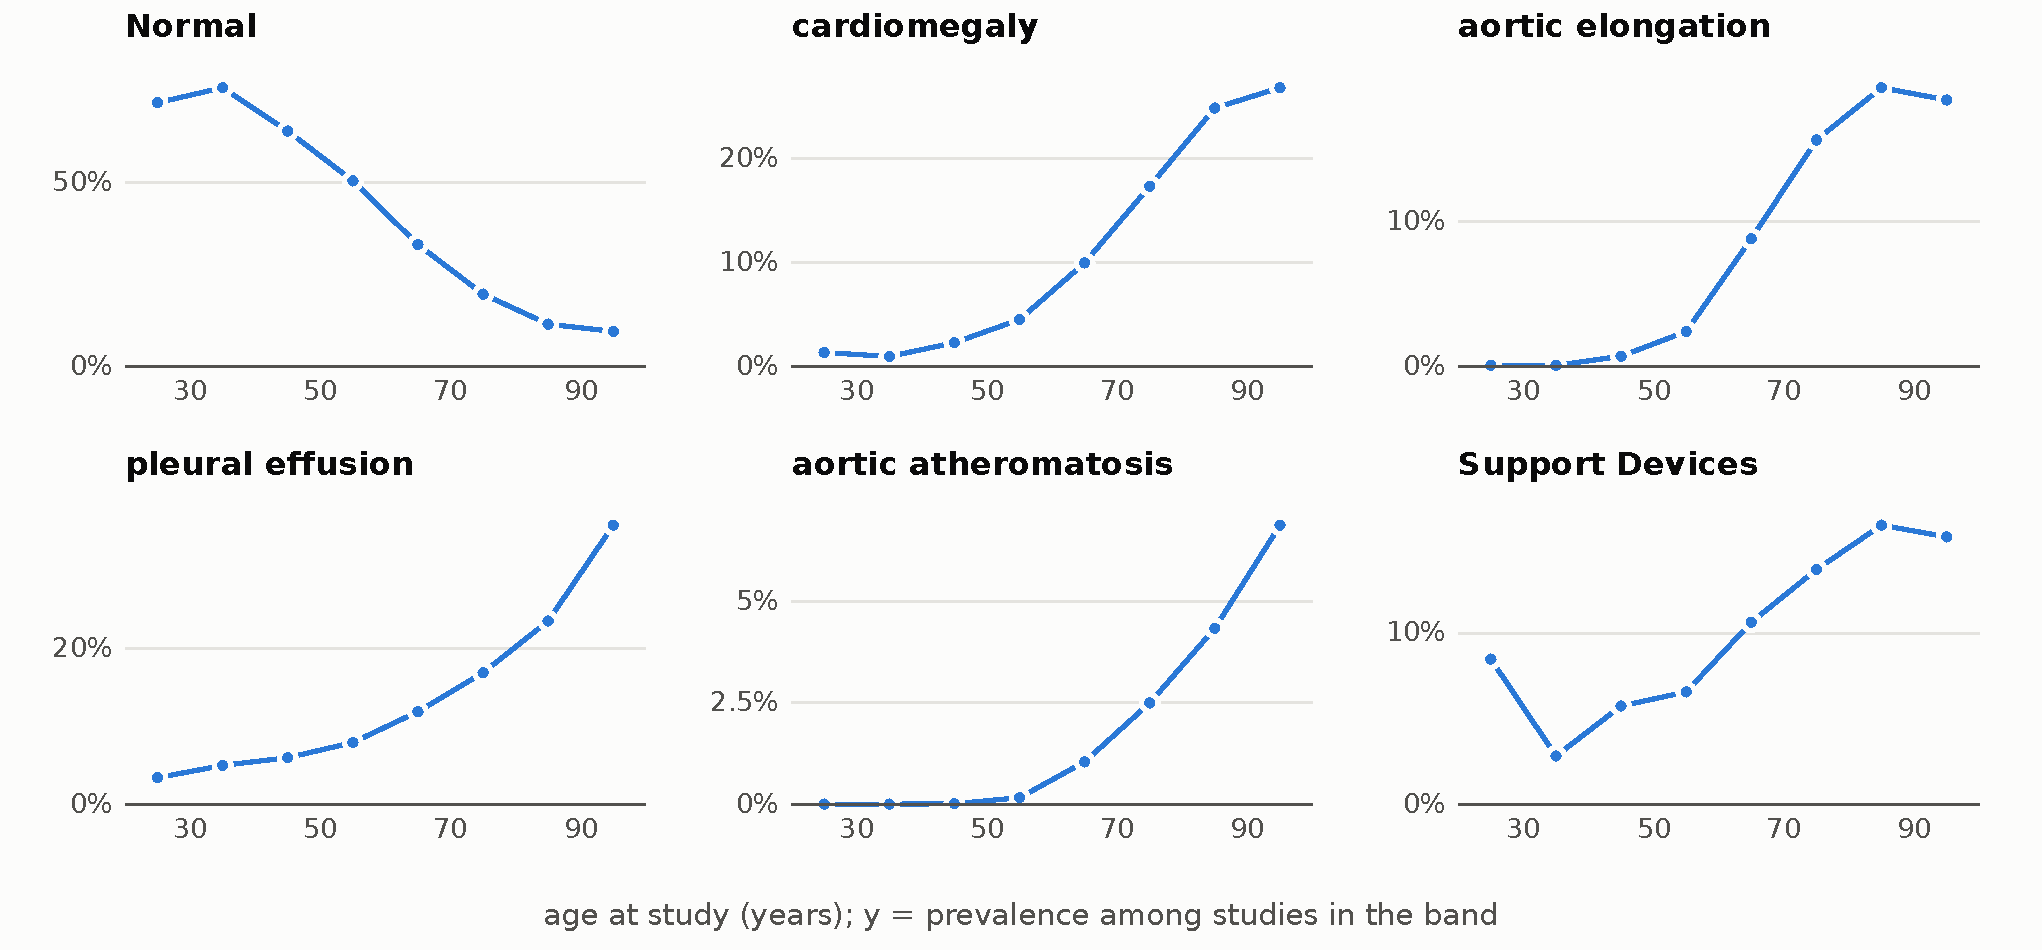
\includegraphics[width=\textwidth]{figures/age_prevalence.pdf}
\caption{Prevalence of six labels by age at study, for the six classes most associated with age. Each point is a 10-year age band of training studies; the vertical axis is the share of studies in the band with the finding. The scales differ between panels.}
\label{fig:age}
\end{figure*}

\begin{figure}[htbp]
\centering
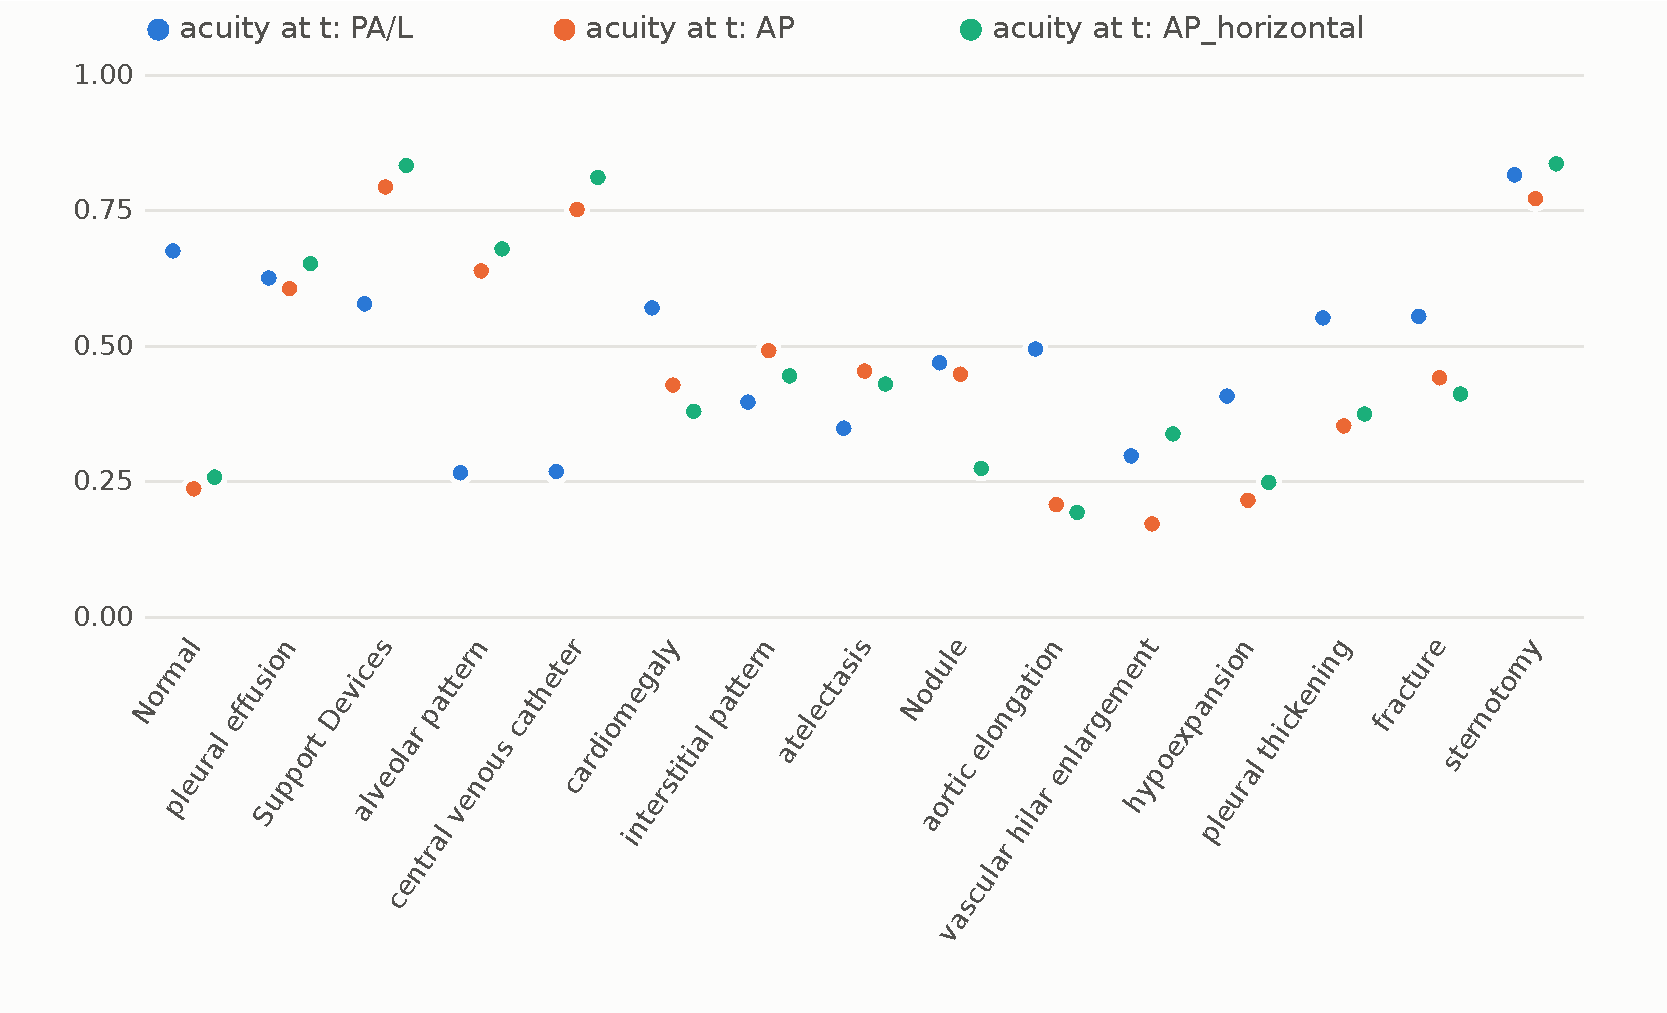
\includegraphics[width=\columnwidth]{figures/persistence_by_acuity.pdf}
\caption{Persistence of findings by the acuity of the later study: the probability that a finding is present at study $t$ given that it was present at study $t-1$ of the same patient (vertical axis), for 15 classes (horizontal axis). Colours give the acuity of study $t$: PA or lateral (blue), AP (orange), AP horizontal (green).}
\label{fig:persist}
\end{figure}

\begin{figure}[htbp]
\centering
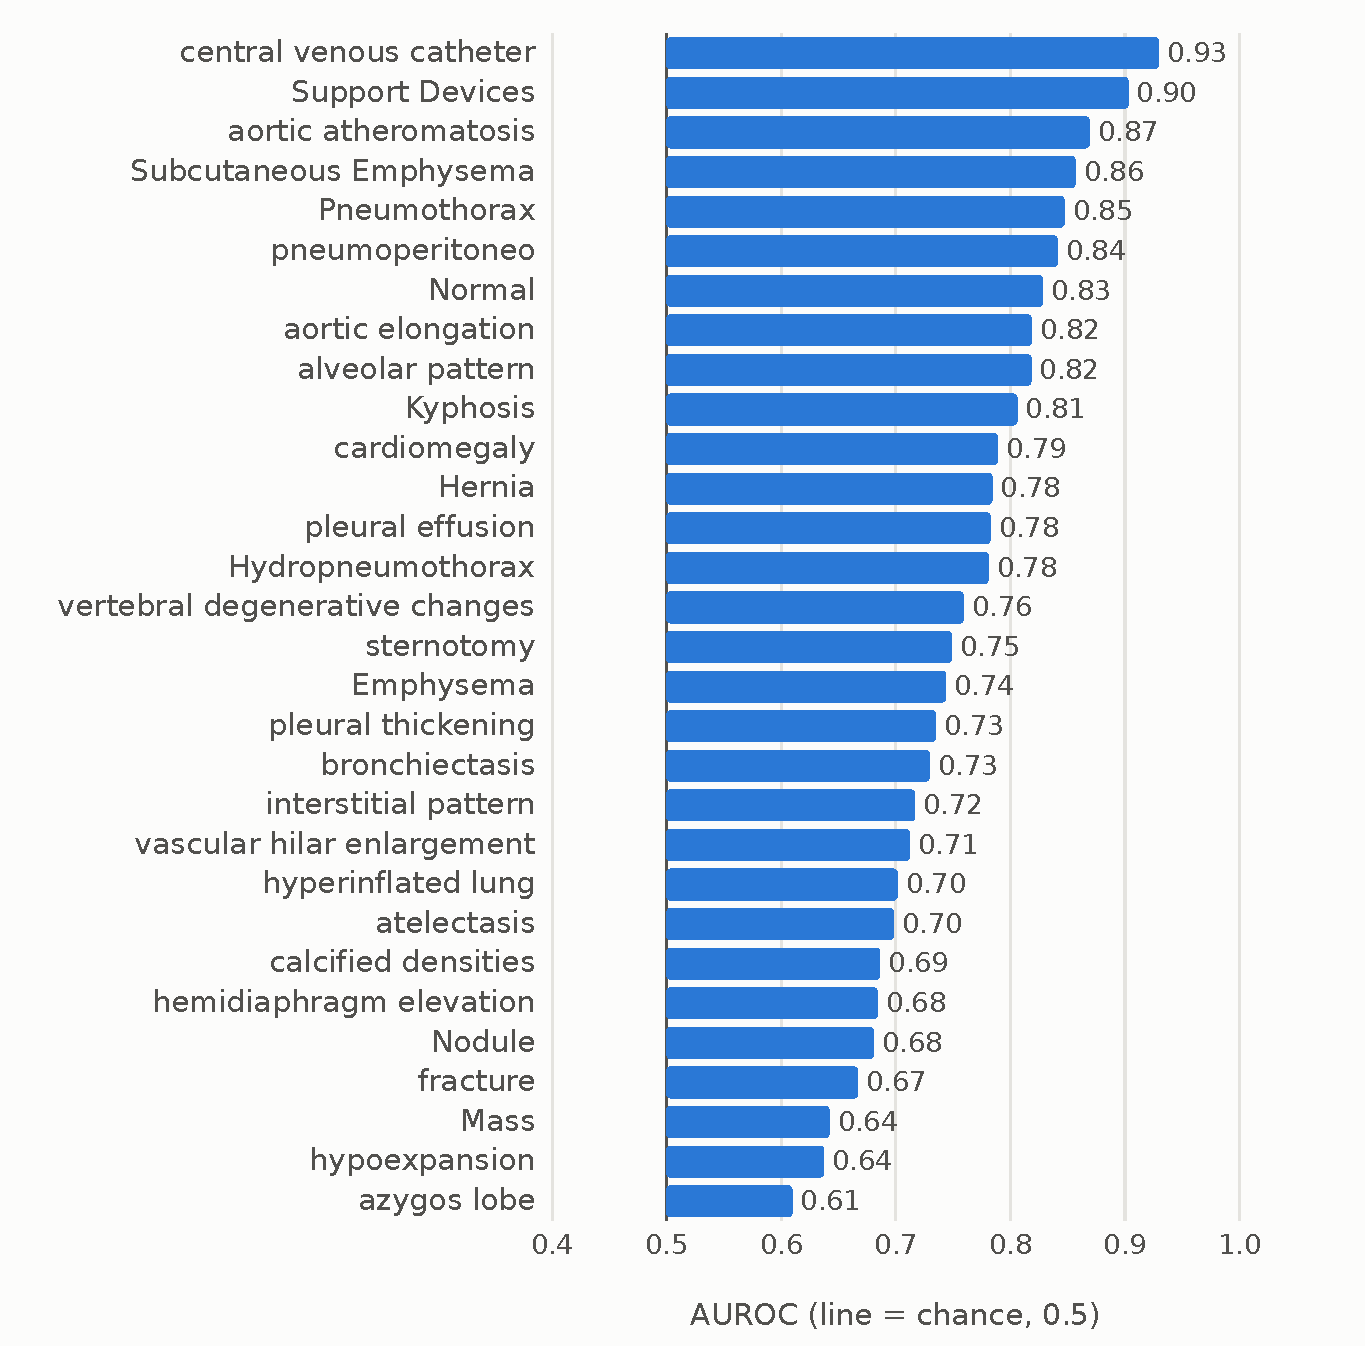
\includegraphics[width=\columnwidth]{figures/metadata_only_auroc.pdf}
\caption{Held-out AUROC of a logistic model that uses metadata only, for each of the 30 classes, sorted from highest to lowest (patient-grouped five-fold cross-validation, training fold). The vertical line marks chance (0.5).}
\label{fig:auroc}
\end{figure}

\subsection{Internal Validation versus the Test Set}
\label{sec:audit}
Checking route (B) required patient identifiers for our own folds, which revealed that our internal validation fold differs from the test set in three ways. The Task~1 test set consists of 3,020 frontal PadChest-GR images (1,620 development, 1,400 test) that each contain at least one target finding, labelled by radiologists and de-duplicated by patient against training~\cite{b14}. Our validation fold, in contrast:
\begin{itemize}
\item \textbf{is not patient-disjoint}: it shares 10,978 patients with the training fold, and 77.0\% of validation images belong to a patient who also appears in training;
\item \textbf{contains lateral views}: 5,234 of 17,270 images;
\item \textbf{uses report-derived labels} rather than radiologist labels.
\end{itemize}

\begin{table*}[htbp]
\caption{Macro mAP (flip TTA) on subsets of the internal validation fold. Seen and unseen refer to whether the image's patient appears in the training fold. The frontal, unseen-patient subset is the closest local proxy for the test set. Each subset is scored over the classes with at least one positive in it.}
\begin{center}
\begin{tabular}{|l|c|c|c|c|c|}
\hline
\textbf{Model} & \textbf{All} & \textbf{Frontal} & \textbf{Lateral} & \textbf{Frontal, seen} & \textbf{Frontal, unseen} \\
 & (17,270) & (11,973) & (5,234) & (8,401) & (3,572) \\
\hline
Greedy-3 ensemble & \textbf{0.4722} & \textbf{0.4968} & \textbf{0.4058} & \textbf{0.5025} & \textbf{0.4752} \\
\hline
1024~px, SWA (seed 86) & 0.4645 & 0.4892 & 0.3954 & 0.4930 & 0.4719 \\
\hline
768~px, SWA (seed 42) & 0.4650 & 0.4875 & 0.3988 & 0.4945 & 0.4706 \\
\hline
896~px, SWA (seed 86) & 0.4578 & 0.4804 & 0.3927 & 0.4838 & 0.4702 \\
\hline
768~px, resolution sweep (seed 86) & 0.4570 & 0.4785 & 0.3894 & 0.4837 & 0.4642 \\
\hline
640~px, resolution sweep (seed 86) & 0.4485 & 0.4717 & 0.3918 & 0.4801 & 0.4514 \\
\hline
512~px, seed sweep (seed 1024) & 0.4480 & 0.4697 & 0.3873 & 0.4750 & 0.4649 \\
\hline
512~px, drop-path 0.1 (seed 86) & 0.4429 & 0.4641 & 0.3838 & 0.4694 & 0.4644 \\
\hline
\end{tabular}
\label{tab:subsets}
\end{center}
\end{table*}

Table~\ref{tab:subsets} scores eight models on each subset. The SWA rows use our final recipe; the other rows are best-epoch checkpoints from earlier sweeps. For the 1024~px SWA model minus the 512~px seed-1024 model, the patient-clustered bootstrap gives $+0.0196$ [$+0.0047$, $+0.0358$] on frontal, seen-patient images and $+0.0074$ [$-0.0200$, $+0.0269$] on frontal, unseen-patient images. Four observations follow.
\begin{enumerate}
\item \textbf{Lateral views lower the headline number.} On frontal images, the view the test set uses, the ensemble scores 0.4968; the full-fold 0.4722 includes laterals at 0.4058.
\item \textbf{The resolution gain is not established on unseen patients.} The 1024-versus-512~px gain is $+0.020$ with an interval that excludes zero on seen patients, but $+0.007$ with an interval that includes zero on unseen patients. The ordering of the resolutions holds only loosely there, and the 640~px model falls below the 512~px one.
\item \textbf{The seen/unseen gap (0.5025 versus 0.4752) is not all memorisation.} Unseen patients have a different case mix: Normal prevalence 0.58 versus 0.35, 1.27 versus 1.57 labels per image, and 90\% versus 63\% frontal. Only a patient-disjoint re-split with matched case mix can separate the two effects.
\item \textbf{The audit is consistent with the known offset} between our internal and leaderboard scores (Stage~1: 0.385 internal, 0.505 on the development leaderboard). The test set is frontal only, and every test image has at least one finding.
\end{enumerate}

\section{Discussion}
\textbf{Why label priors do not help here.} ML-Decoder's query self-attention is itself a row-stochastic $30 \times 30$ mixing over labels. It is recomputed for every image, operates on 768-dimensional label embeddings, and is repeated over 8 heads in each of 2 blocks. The Markov layer adds one global matrix applied to probabilities. For a ranking metric, a global matrix can only move scores in the same direction for every image with similar predicted findings, which is what the post-hoc results show. The trainable layer was free to use or ignore the prior, and it stayed near the identity, with every gate below 0.062 in magnitude. We read this as the network finding little in a global prior that its decoder had not already captured. With a single seed and a four-epoch schedule, this is suggestive rather than conclusive.

\textbf{What patient history adds.} A prior that conditions on the previous state does help when that state exists: H4 gains about $+0.04$ mAP on images with a prior study, and fusing it after the classifier is as good as training it into the network. The gain is not a label-graph effect, since the within-state couplings were never selected. It comes mostly from the previous report, and the metadata that were meant to refine it add nothing. The caveats are those of the setup: labels are extracted from reports, the validation fold shares patients with the training fold, the filtered-mode history of training images is in-sample, and there is one validation fold. The result applies to a deployment with prior reports, not to the test set.

\textbf{What the challenge winners did instead.} None of the top CXR-LT 2024 or 2026 Task~1 solutions used Markov, label-graph or patient-history modelling (Table~\ref{tab:winners}). The ingredient the winners share and we lack is chest-X-ray-domain pretraining. The challenge rules allow \emph{``models pretrained \ldots\ on external CXR datasets that do not overlap with the CXR-LT evaluation images''}, but forbid using \emph{``hidden test labels, manually relabel[ing] evaluation images, or \ldots\ external annotations overlapping with the CXR-LT evaluation sets''}~\cite{b14}. MIMIC-CXR pretraining is therefore legitimate. The public PadChest-GR labels~\cite{b10} are the evaluation annotations and must not be used, even for tuning.

\begin{table*}[htbp]
\caption{Key ingredients of the top published CXR-LT Task~1 solutions~\cite{b14,b15,b16}.}
\begin{center}
\begin{tabular}{|c|l|p{10.2cm}|c|}
\hline
\textbf{Year} & \textbf{Team} & \textbf{Key ingredients} & \textbf{mAP} \\
\hline
2026 & 1st~\cite{b15} & ConvNeXtV2-B pretrained on MIMIC-CXR, 512~px, Distribution-Balanced loss (effective-number reweighting and a positive logit margin), class-aware sampling, Normal-gating, weighted checkpoint ensemble, TTA & 0.585 \\
\hline
2026 & 2nd & ConvNeXtV2 and SwinV2-T, 512~px, PCAM pretraining, strong augmentation, ensemble, TTA & 0.483 \\
\hline
2026 & 3rd (ours~\cite{b12}) & ConvNeXt, 384~px, ImageNet initialisation, Asymmetric Loss with auxiliary loss, Mixture-of-Experts Stage~2, TTA & 0.460 \\
\hline
2024 & several~\cite{b16} & Chest-X-ray-domain pretraining (e.g.\ DINOv2 ViT-L on 710k chest X-rays; NIH, CheXpert, VinDr), ML-Decoder heads, multi-view and multi-resolution ensembles, synthetic tail data & --- \\
\hline
\end{tabular}
\label{tab:winners}
\end{center}
\end{table*}

\textbf{Recommendations.}
\begin{enumerate}
\item Re-anchor internal evaluation on a leaderboard-like proxy: a patient-disjoint, frontal-only validation fold, ideally restricted to images with at least one finding. Reporting the frontal, unseen-patient subset of Table~\ref{tab:subsets} for every new checkpoint is a cheap first step; a proper patient-disjoint re-split of the same images is the full fix.
\item Re-check the resolution conclusion on that proxy before spending more compute on inputs of 896~px and above.
\item Pursue chest-X-ray-domain pretraining. Our Stage~1 starts from ImageNet, whereas the 2026 winner started from MIMIC-CXR.
\item Drop label-graph Markov variants for Task~1. Use a patient-history HMM only where prior reports exist, with calibrated late fusion (H1) as the starting point.
\end{enumerate}

\section{Conclusion}
We tested whether Markov-chain priors help long-tailed multi-label chest X-ray classification on CXR-LT 2026 Task~1, along both available state sequences. Over the label graph, a fixed co-occurrence prior, the challenge winner's Normal-gating prior, and a trainable identity-initialised Markov layer all failed to improve a model whose ML-Decoder head already mixes labels per image. Over a patient's studies, a hidden Markov model has no history to condition on at test time, by the challenge's design and data-use terms. In a longitudinal simulation, a post-prediction patient HMM gains about $+0.04$ mAP on images with a prior study, matches a network fed the same prior, and owes most of the gain to the previous report (image-only history gives $+0.009$); the simplest calibrated chain is as good as the richest, and the leaderboard effect is 0. The investigation instead showed that our internal validation fold, which is not patient-disjoint and includes lateral views, is a weak proxy for the frontal, patient-disjoint test set, and that a resolution gain measured on it is not significant on unseen patients. We report these negative results so that others working on CXR-LT can skip label-graph Markov priors and evaluate on a patient-disjoint, frontal proxy from the start.

\appendix
\section*{Reproducibility}
\begin{itemize}
\item \textbf{Post-hoc results} (Tables~\ref{tab:smoothing}, \ref{tab:gating} and~\ref{tab:subsets}, and the patient counts) are printed by \path{analysis/markov_check.py} from the cached flip-TTA probabilities in \path{analysis/out/probs_w01_flip/}. The rebuilt validation row order is stored in \path{analysis/out/val_key_order.npy}. The reverse gate, the single-model gating check and the patient-clustered bootstrap were run separately and are not part of that script.
\item \textbf{Trainable layer:} \path{train/markov_layer.py} and \path{train/train_2_v4.py}. The variants are Slurm jobs 49063 (mk1), 49064 (mk2) and 49065 (mk1fix); the matched baseline is job 49000.
\item \textbf{Post-prediction HMM} (Table~\ref{tab:hmm}): \path{analysis/markov_hmm.py} (model), \path{analysis/markov_hmm_check.py} (arms, cross-fitting, bootstrap) and \path{analysis/patient_meta.py} (metadata whitelist), run as Slurm job 49445 (output in \path{analysis/out/markov_hmm/}). The metadata analysis of Section~\ref{sec:metaeda} is \path{analysis/metadata_eda.py}. An earlier observed-mode run (job 49424) gives identical H0 and H1 and differs by at most 0.0014 mAP for the logistic-prior arms, because float differences between CPU nodes occasionally change a tied grid weight.
\item \textbf{Patient grouping} must use the original PadChest metadata read as strings. The \path{PatientID} column of the filtered challenge CSV is stored as a rounded float, which merges distinct patients.
\end{itemize}

\section*{Acknowledgment}
The authors thank the organizers of the ISBI 2026 CXR-LT challenge for providing the benchmark dataset and evaluation infrastructure.

\begin{thebibliography}{00}
\bibitem{b1} Zhuang Liu, Hanzi Mao, Chao-Yuan Wu, Christoph Feichtenhofer, Trevor Darrell, and Saining Xie, ``A ConvNet for the 2020s,'' in IEEE/CVF Conference on Computer Vision and Pattern Recognition, CVPR 2022, New Orleans, LA, USA, June 18-24, 2022, pp. 11966--11976, IEEE.
\bibitem{b2} Tal Ridnik, Gilad Sharir, Avi Ben-Cohen, Emanuel Ben-Baruch, and Asaf Noy, ``ML-Decoder: Scalable and versatile classification head,'' arXiv:2111.12933, 2021.
\bibitem{b3} Tal Ridnik, Emanuel Ben Baruch, Nadav Zamir, Asaf Noy, Itamar Friedman, Matan Protter, and Lihi Zelnik-Manor, ``Asymmetric loss for multi-label classification,'' in 2021 IEEE/CVF International Conference on Computer Vision, ICCV 2021, Montreal, QC, Canada, October 10-17, 2021, pp. 82--91, IEEE.
\bibitem{b6} Xun Wang, Haozhi Zhang, Weilin Huang, and Matthew R. Scott, ``Cross-batch memory for embedding learning,'' in IEEE/CVF Conference on Computer Vision and Pattern Recognition, CVPR 2020, Seattle, WA, USA, June 13-19, 2020, IEEE.
\bibitem{b9} Aurelia Bustos, Antonio Pertusa, Jose-Maria Salinas, and Maria de la Iglesia-Vaya, ``Padchest: A large chest x-ray image dataset with multi-label annotated reports,'' Medical Image Analysis, vol. 66, pp. 101797, 2020.
\bibitem{b10} Daniel Coelho de Castro, Aurelia Bustos, Shruthi Bannur, Stephanie L. Hyland, Kenza Bouzid, Maria Teodora Wetscherek, Maria Dolores S\'anchez-Valverde, Lara Jaques-P\'erez, Lourdes P\'erez-Rodr\'iguez, Kenji Takeda, Jos\'e Mar\'ia Salinas-Serrano, Javier Alvarez-Valle, Joaqu\'in Galant-Herrero, and Antonio Pertusa, ``Padchest-gr: A bilingual chest x-ray dataset for grounded radiology report generation,'' NEJM AI, vol. 2, no. 7, June 2025.
\bibitem{b11} Hexin Dong, Yi Lin, Pengyu Zhou, Xuan Zhong Feng, Alan Clint Legasto, Mingquan Lin, Hao Chen, Yuzhe Yang, George Shih, and Yifan Peng, ``Overview of the CXR-LT 2026 challenge: Multi-center long-tailed and zero shot chest X-ray classification,'' arXiv:2602.22092, 2026.
\bibitem{b12} Huy Le Pham, Khoa Ha Anh, Nguyen-Thanh-Thao Vo, Ky Trung Nguyen, Chau Ly Thi Huyen, Hien Q. Ta, and Thang Doan Van, ``An efficient framework for long-tailed and multi-label classification on chest X-rays,'' ISBI 2026 Task 1, 2026.
\bibitem{b13} Nicolas Carion, Francisco Massa, Gabriel Synnaeve, Nicolas Usunier, Alexander Kirillov, and Sergey Zagoruyko, ``End-to-end object detection with transformers,'' in Computer Vision - ECCV 2020 - 16th European Conference, Glasgow, UK, August 23-28, 2020, Proceedings, Part I, vol. 12346 of Lecture Notes in Computer Science, pp. 213--229, Springer.
\bibitem{b14} Hexin Dong, Yi Lin, Pengyu Zhou, \textit{et al.}, ``CXR-LT 2026 challenge: Multi-center long-tailed and zero shot chest X-ray classification,'' arXiv:2604.15555, 2026.
\bibitem{b15} Ha-Hieu Pham, Hai-Dang Nguyen, Thanh-Huy Nguyen, Min Xu, Ulas Bagci, Trung-Nghia Le, and Huy-Hieu Pham, ``Handling supervision scarcity in chest X-ray classification: Long-tailed and zero-shot learning,'' in 2026 IEEE 23rd International Symposium on Biomedical Imaging (ISBI), 2026, arXiv:2602.13430.
\bibitem{b16} Mingquan Lin, Gregory Holste, Song Wang, \textit{et al.}, ``CXR-LT 2024: A MICCAI challenge on long-tailed, multi-label, and zero-shot disease classification from chest X-ray,'' arXiv:2506.07984, 2025.
\bibitem{b17} Bingzhi Chen, Jinxing Li, Guangming Lu, Hongbing Yu, and David Zhang, ``Label co-occurrence learning with graph convolutional networks for multi-label chest X-ray image classification,'' IEEE Journal of Biomedical and Health Informatics, vol. 24, no. 8, pp. 2292--2302, 2020.
\bibitem{b18} Jesse Read, Bernhard Pfahringer, Geoff Holmes, and Eibe Frank, ``Classifier chains for multi-label classification,'' Machine Learning, vol. 85, no. 3, pp. 333--359, 2011.
\bibitem{b19} Jiang Wang, Yi Yang, Junhua Mao, Zhiheng Huang, Chang Huang, and Wei Xu, ``CNN-RNN: A unified framework for multi-label image classification,'' in 2016 IEEE Conference on Computer Vision and Pattern Recognition (CVPR), 2016, pp. 2285--2294.
\bibitem{b20} Shruthi Bannur, Stephanie Hyland, Qianchu Liu, \textit{et al.}, ``Learning to exploit temporal structure for biomedical vision-language processing,'' arXiv:2301.04558, 2023.
\bibitem{b21} Eva Prakash, Yunhe Gao, Chong Wang, \textit{et al.}, ``CheXTemporal: A dataset for temporally-grounded reasoning in chest radiography,'' arXiv:2605.11304, 2026.
\bibitem{b22} Iulian Emil Tampu, Anders Eklund, and Neda Haj-Hosseini, ``Inflation of test accuracy due to data leakage in deep learning-based classification of OCT images,'' Scientific Data, vol. 9, 2022.
\bibitem{b23} Tong Wu, Qingqiu Huang, Ziwei Liu, Yu Wang, and Dahua Lin, ``Distribution-balanced loss for multi-label classification in long-tailed datasets,'' in Computer Vision -- ECCV 2020, Lecture Notes in Computer Science, pp. 162--178, Springer, 2020.
\bibitem{b24} Xavier Boyen and Daphne Koller, ``Tractable inference for complex stochastic processes,'' in Proceedings of the Fourteenth Conference on Uncertainty in Artificial Intelligence (UAI), 1998, pp. 33--42.
\end{thebibliography}

\end{document}
